\documentclass[usenatbib]{mn2e}

\usepackage{amsmath}
\usepackage{graphicx}
\usepackage{epstopdf}
\usepackage{multicol}

\title{Microlensing as a possible probe of the internal structure of quasars}

\author[Tomozeiu et al]{Mihai Tomozeiu$^{1,2}$,Irshad Mohammed,$^1$ Manuel Rabold$^2$,
\newauthor
Prasenjit Saha,$^1$ and Joachim Wambsgans$^3$\\
$^1${Physik-Institut, University of Zurich, Winterthurerstrasse 190,
  8057 Zurich, Switzerland} \\
$^2${Institute for Computational Science, University of Zurich,
  Winterthurerstrasse 190, 8057 Zurich, Switzerland} \\
$^3${Zentrum f\"ur Astronomie der Universi\"at Heidelberg,
  M\"onchhofstrasse 12--14, 69120 Heidelberg, Germany}
}

\begin{document}

\maketitle

\begin{abstract}

In quasars that have been lensed by galaxies, the point-like images
sometimes show sharp brightness variations (microlensing).  These
brightness changes are associated with the innermost region of the
quasar passing behind a complicated pattern of caustics due to the
stars in the lensing galaxy.  In this paper, we study whether the
universal properties of optical caustics could enable extraction of
shape information about the central engine of quasars.  We present a
toy model with a crescent-shaped source crossing a fold caustic.  The
silhouette of a black hole over an accretion disk tends to produce
roughly crescent sources.  When a crescent source crosses a fold
caustic, the resulting light curve is noticeably different from the
case of a disc or Gaussian source.  The crescent parameters, apart
from one degeneracy, can be recovered.
\end{abstract}


\begin{keywords}
Supermassive black holes, microlensing, quasars.
\end{keywords}




%%%%%%%%%%%%%%%%%%%%%%%%%%%%%%%%%%%%%%%%%%%%%%%%%%%%%%%%%%%%%%%%%%%%%%%%%%
\section{introduction}
More than half a century after their discovery, quasars still maintain the interest of a productive part of the astrophysical community. Although several mechanisms have been proposed 
to explain how such systems function, a single mechanism is widely accepted at the present time. The model was first proposed by \cite{1964ApJ...140..796S}, followed by \cite{1964SPhD....9..246Z} in the same year and \cite{1969Natur.223..690L} five years later. The present name of the model is the Super-Massive Black Hole (SMBH) paradigm.\\

According to the paradigm, the object is powered through the accretion of matter from the proximal environment into the black hole. The radiation emitted excites the surrounding medium which becomes detectable as the narrow line regions,
broad band regions and torus. Moreover, in the direction perpendicular to the accretion disk, where the medium is more transparent, jets will appear. When the medium between and observer and such an object is transparent a quasar can be observed (citation). In other words an active galactic nucleus (AGN) with one of the poles orientated towards Earth would be detected as a quasar by an observer. \\

Through extensive observations done in the past 50 years, an important part of the assumptions and details  regarding the mechanism have been confirmed and uncovered. Still, the black hole shadow and the surrounding luminous accreting material (the black hole silouette) remains to be probed. Advancements in the very long baseline interferometer observations have made possible since 2007, the detection of structures of a few Schwarzschild radii at the Sagitarius A object at the center of our galaxy \citep{2008JPhCS.131a2055D}. Furthermore, jet launching structure near the supermasve black hole in M87 were resolved with the same observation tool \citep{2012Sci...338..355D}. With all the advancement, the current number of baselines does not allow the direct generation of images from the observations still it does allow the fitting of the data to predefined models \citep{2013MNRAS.434..765K}.


A whole range of models have been applied starting from simple geometric models to more complex, physically sensible models (Doeleman et al 2008, Fish et al 2011, Broderick et al 2011, Moscibrodzka et al 2009, Dexter 2010 and others). A significant fraction of the later models predict a crescent shaped silouette of the black hole. This motivated \cite{2013MNRAS.434..765K} to use a simple geometric crescent model to fit the data. The succesfull results encouraged the authors to speculate that the shadow of the black hole will be observed in the near fututre with the previously mentioned observation method. \\


Hundreds of thousands of quasars have been detected up to date, mainly from the Sloan Digital Sky Survey. The great majority of them present a redshift larger than 2.15 of their spectra (Paris et al 20Nov 2013 SDSS catalogue). Therefore the typical distance to the objects is in the order of gigaparsecs  or above. A value that is orders of magnitude larger than the distance to M87. Direct observation of the black hole silouette of quasars require significant technological advances. We argue in the present paper
 that one can probe and study the black hole shadow and its proximal environment belonging to a quasar without having to resolve sub-event horizon scales. We consider that this is possible by analyzing the data from microlensing-events.  Moreover, unlike with the few nearby AGNs, the study of the very large quasar population allows for the statistical refinement of the global properties of AGN by highlighting any particular
characteristic that is present only in SGA* and M87 central region. Furthermore, by probing the event-horizon-scale inner regions of a large number of objects will facilitate the study of the evolution of the previously mentioned region.     
     
Gravitational microlensing of QSOs have been predicted as early as 1981 when \cite{1981ApJ...243..140G} suggested that ''if haloes of galaxies were composed of stars with masses less than  0.1 $M_{sol}$, then these stars acting as individual lenses whould produce fluctuations of the order of 
unity in the intensities of the QSO images on time scales of 1 -14 years '' (Gott 1981). What creates the magnification event is the relative and independent motion of the lens and source with respect to the observer. Since the respective lens is surrounded by similar objects one would expect to observe during a long enough time interval
multiple microlensing events of the same source, the QSO. The sequential alignment of the source and observer with different lensing objects will result in an aparently random increase of the QSO light flux analogous to the scintilation events in a meter of radioactivity.

Estimates of the Einstein radius for the particular case of a QSO at redshift 2 lensed by a compact stellar mass object at redshift 0.5 was found to be $10^-6 \sqrt{M/M_{sol}} arcsec$ \citep{2001PASA...18..207W}. The Schwarzschild radius of the Sgr A* black hole, situated at 8 kpc from Earth \citep{1993ARA&A..31..345R} spans an angle of 10 microarcsec on the sky \citep{2008JPhCS.131a2055D}. If the quasars observed at z =2 would have similar linear sizes, the aparent size of the  luminous part of the QSO would be many orders of magnitude below the 1 microarcsec level. Therefore the aparent size would be significantly smaller than the corresponding Einstein radius of a solar mass lens. 
The magnitude differences between the Einstein angle and the aparrent size of the bright part of the QSO motivates the introduction in the first part of the paper of simplified models for     
calculating the lightcurves of QSO magnification events. The simplified models are introduced in the theory section of the present paper. In the theory (II) section of the present article with an introduction to the basic microlensing theory in which we present the general microlensing equation followed by the concept of magnification. We underline that for the particular case of micro gravitational lensing,
the images are not resolved and thus the magnifications of each images contribute to a total magnification. Furthermore, the concept of critical curves and caustics are introduced. Afterwards we focus on a particular singularity, namely the fold singularity. We choose to study events related to the previously mentioned singularity since the magnification events caused by the crossing of such boundaries are most probable. A quick inspection of figure 1 by the reader should motivate the previous statement. 
In continuation we introduce the commonly used result involving the magnification of a point-like source near a fold singularity. Namely that the magnification is aproximately linear outside the caustic and decreases from infinity with the square root of the distance to the boundary when inside the caustic.  
In the last section of the Introduction (II) we present the general equations for estimating the flux received from an extended source near a fold. The only elements required to compute the flux as a function of time are the two dimensional brightness function of the object and the magnification of a point-like source. One of the core
assumptions made when developing the simple models is that the einstein angle is orders of magnitude greater than the apparent size of the source. Due to this assumption one can imagine the caustic as an infinite wall to be crossed by the source as presented in figure 2. The consequence of the limit is that the information regarding the profiles of the source along any direction parallel to the boundary value is reduced to the corresponding integral value. The effect allows the introduction of a one dimensional flux function, which is the two dimensional flux integrated along the axis paralel to the boundary. The one dimensional profile contains exhaustively all the information that can be extracted  from the lens generated light-curve \\

\begin{figure}
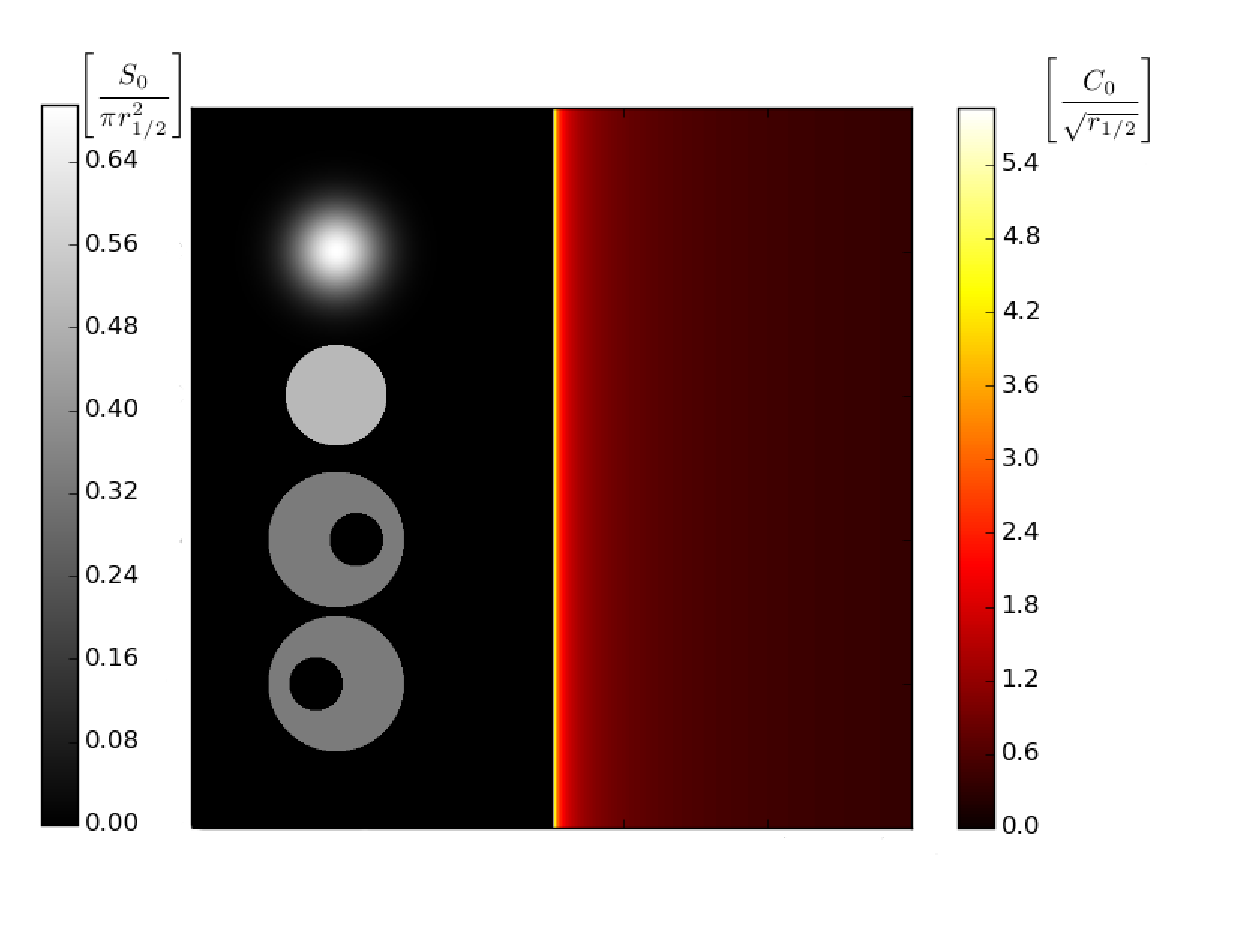
\includegraphics[width = .8\textwidth]{plots/infinite_fold.eps}
\caption{\label{fig:infinite_fold}  Source profiles and magnification map for an infinite fold. Objects have the same $S_{0}$ and $r_{1/2}$ }
\end{figure}




In the third section we introduce the three source profiles used in our models and simulations. We start with two commonly used and simple sources. Namely the gaussian brightness distribution and the constant intensity disk. In addition we use a geometric crescent-shaped source effectively the same as the one introduced by \citep{2013MNRAS.434..765K} with constant surface brightness. \\
The fourth section contains the results of our simplified models calculations, including the numerical equation for lightcurve calculations and the corresponding plots. In order to facilitate comparison bewteen the lightcurves of the three distinct sources, we constrain the luminosity and half-light radius of all sources to have the same value.    
       
We continue to the second part of the paper, where we have advanced the level of complexity of our models. Using the Wambsganss gravitational lensing code (citation) a realistic magnification map is generated. The magnification map replaces the simplified magnification function used previously.  \\
The numerical method, hierachical tree structure and backwards reatracing, underlying the microlensing code is treated in section five. Aside from a basic review of the physical and numerical principles of the code, the description of its generalization from disk shaped source images to crescent ones can be found here as well. Further, the mass distribution in the lens plane, chosen to produce the magnification map used in this analysis, is introduced and motivated.   



\section{Theory}

We start by introducing in a succinct manner the gravitational lensing
theory that is relevant for microlensing in general and for the scope
of the present paper in particular.  More detailed presentation of the
theory can be found in several references, such as
\cite{2001stgl.book.....P}.

\subsection{Microlensing essentials}

The gravitational lens equation
\begin{equation}
\vec\beta = \vec\theta - \vec\alpha(\vec\theta)
\label{eqn:lens}
\end{equation}
relates the apparent sky position $\vec\theta$ of a light source to
its true but unobservable sky position $\vec\beta$ through the bending
angle $\vec\alpha$.  The latter is an integral 
\begin{equation}
\vec\alpha = (1+z_{_L})\frac{D_S-D_L}{D_SD_L} \frac{4G}{c^2}
\int \Sigma(\vec\theta')
\frac{\vec\theta-\vec\theta'}{|\vec\theta-\vec\theta'|^2}\,
d^2\vec\theta'
\label{eqn:alpha}
\end{equation}
depending on the projected density $\Sigma(\vec\theta)$ (kg/steradian)
of the lens, the lens redshift $z_{_L}$ and the comoving distances
$D_L$ and $D_S$ to the lens and source.  The derivative of the
apparent position with respect to the source position
\begin{equation}
M(\vec\theta) =
\left(\frac{\partial\beta}{\partial\theta}\right)^{-1}
\label{eqn:magnif-matrix}
\end{equation}
is known as the magnification matrix, and its determinant
\begin{equation}
\mu(\vec\theta) = \det|M(\vec\theta)|
\end{equation}
is the brightness amplification of an image of a point source.  In
other words, the source will brighten or dim according to whether
$\mu(\vec\theta)$ is more or less than unity.  If there are multiple
mages at distinct but not observationally resolved $\vec\theta_i$ from
the same $\vec\beta$, a total brightness amplification
of\begin{equation} \mu_{\rm total} = \sum_{i} \mu(\vec\theta_i)
\end{equation}
applies. It is possible for the magnification to become formally
infinite, as a result of an eigenvalues of the magnification matrix
(\ref{eqn:magnif-matrix}) becoming infinite.  This generically happens
on curves on the $\vec\theta$ plane, known as {\em critical curves}.
Mapping a critical curve to the source plane, through the lens
equation (\ref{eqn:lens}), to the source plane $\vec\beta$ gives the
so-called caustics.  Caustics can appear in optical system, not just
gravitational lensing.  For a point source, caustics are singularities
of the magnification; for finite-size sources caustics correspond to
high and sharply changing magnification.

Caustics are important in all forms of lensing with multiple images,
but they have a special significance for lens quasars, first pointed
out by \cite{1979Natur.282..561C}.  The granularity of the mass
distribution $\Sigma(\vec\theta)$ due to individual stars produces a
caustic network on the scale of $\sqrt{GM_\odot D_L/c^2}$ or
micro-arcsec.  Extended sources wash out this micro-caustic structure,
but the optical-continuum source of quasars is even smaller.  Hence
sharp changes in the brightness of lensed quasars are observable, as
they cross the micro-caustics \citep[e.g.,][]{2012A&A...544A..62S}.

\begin{figure}
\centering
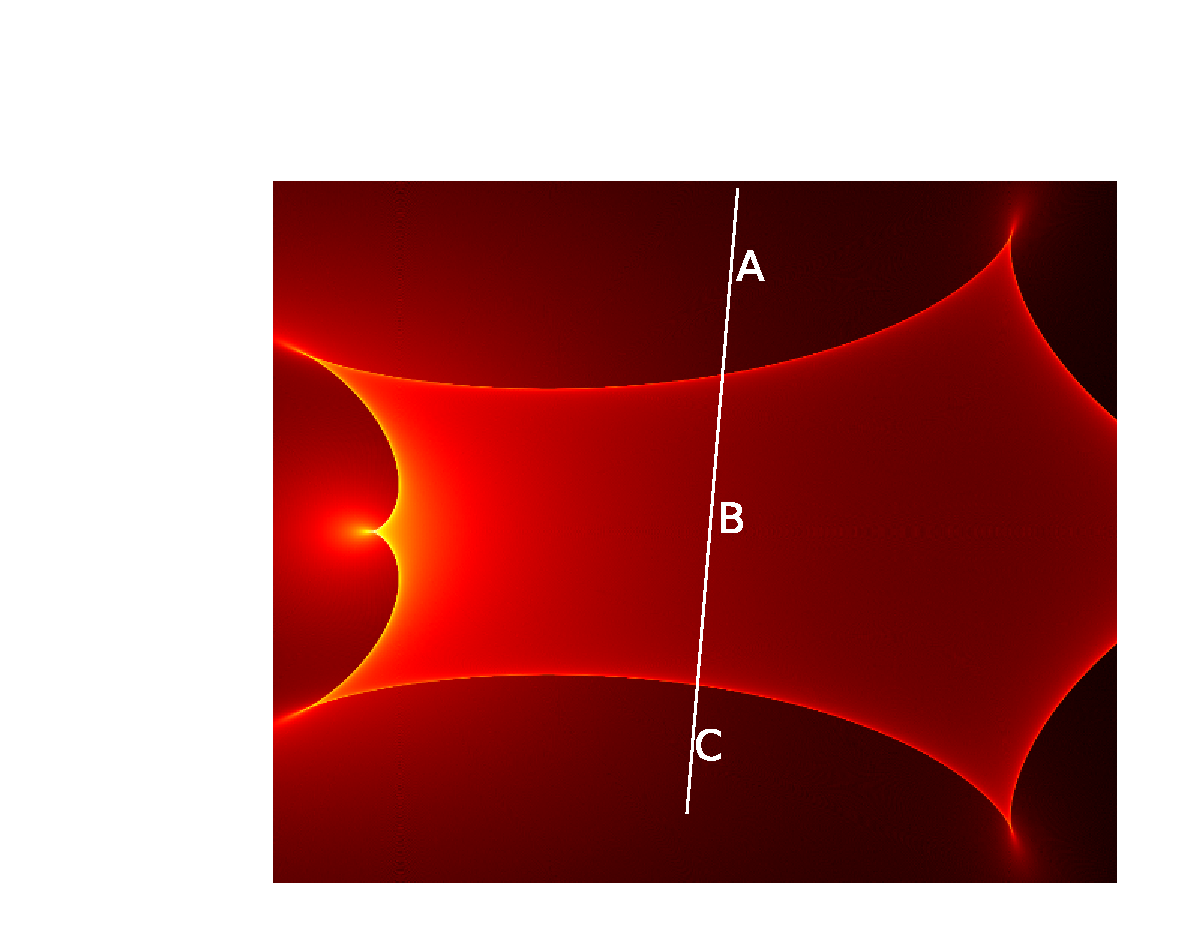
\includegraphics[width=0.9\hsize,bb=0 0 576 432
		]{plots/IRIS567_path_2.eps}
\caption{\label{fig:magnification_map} Magnification map used in the second part of the presented work. The white line marks the trajectory of the center of the sources for which the lightcurves presented in figure 12 are generated.}
\end{figure}






\subsection{Magnification near a fold caustic}

A simple example of a caustic network is shown in
Figure~\ref{fig:magnification_map}.  There are two general categories
of caustics in gravitational lensing, cusps and fold, and examples of
both kinds can be seen in this figure.  Magnification near a caustic
has universal properties, independent of the system and has been
extensively studied
\citep{1986ApJ...310..568B,1992A&A...260....1S,2002ApJ...574..970G,2002ApJ...580..468G}.
In particular, at distance $p$ from a fold caustic
\begin {equation}
 \mu(p) = \mu_0 + C_0 \frac{1}{\sqrt{p}} \Theta(p).
\end {equation}
Here the magnification of a point source near a caustic is equal to
the sum of the magnification due to other reasons $\mu_0$, assumed to
be locally constant, and a decrease with the square root of the
distance from the fold. The later term becomes activated only after
the source enters the region interior to the caustic curves when the
values of the stepfunction $\Theta(p)$ become unity. The
proportionality constant $C_0$ depends on the local conditions in the
vicinity of the caustic.

A source of arbitrary shape can be described by a two dimensional brightness function $S_{2D}(p - p_s, q - q_s)$ defined for a coordinate system $p,q$ where $p_s, q_s$ denote the coordinates of the center of source.

\begin{figure}
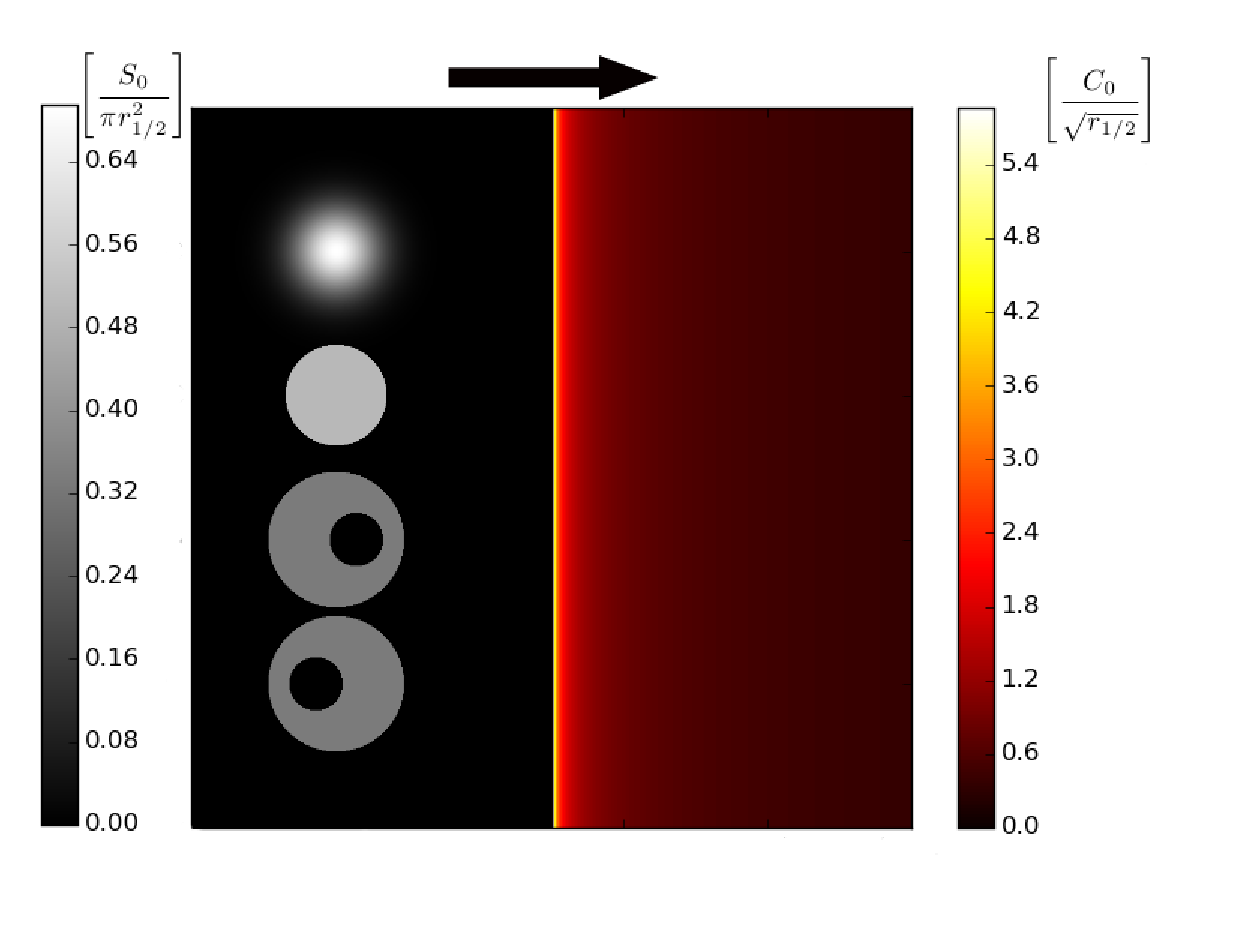
\includegraphics[width = .49\textwidth]{plots/infinite_fold_ar.eps}
\caption{\label{fig:infinite_fold} Source profiles for Gaussian, disk,
  crescents (right) and magnification map for an infinite fold
  (left). Objects have the same $S_{0}$ and $r_{1/2}$. The black arrow marks the direction of motion of the
sources relative to the caustic.}
\end{figure}

For a microlensing event the lightcurve can be written for an
undefined source shape as:
\begin{equation}
 F(t) = \int_{-\infty}^\infty \int_{-\infty}^\infty S_{2D}(p-p_s(t), q-q_s(t)) \mu_t(p) \mathrm{d}q \mathrm{d}p
 \label{eqn:ft2d}
\end{equation}
In order to build the previous equation we have considered that the
time dependency of the flux $F$ is given only by the motion of the
source with respect to a fixed caustic. Therefore the only time
dependent quantities in the right hand side of the equation are the
coordinates of the center of the source $p_s,q_s$ and by construct
$S_{2D}$.

Due to the choice of the coordinate system the amplification factor has no dependence on the $q$ coordinate. The previous equation can be rewritten as:

\begin{equation}
 F(t) 
= \int_{-\infty}^\infty  \mu_t(p) S_{1D}\left(p-p_s(t)\right) \mathrm{d}p,
\label{eqn:ft}
\end{equation}
\\
where we have defined the one dimensional flux function as:
\begin{equation}
 S_{1D}(p-p_s(t)) = \int_{-\infty}^\infty S_{2D}(p-p_s(t), q-q_s(t)) \mathrm{d}q
\end{equation}

This representation is a valid approximation only when the apparent size of the source is much smaller than the corresponding Einstein angle of the lens. In this context 
all the information about the source shape and brightness that can be contained in the lightcurve is exhaustively given by the 1D flux function.
In other words, if two sources with different $S_{2D}$ have the same $S_{1D}$ they cannot be distinguished by studying their lightcurves.
 
 
\section{Models for extended sources}

In the present study we are analysing three types of sources with different surface brightness: 
\begin{enumerate}
 \renewcommand{\theenumi}{(\arabic{enumi})}
  \item a rotationally symmetric source with a bivariate gaussian surface brightness distribution,
  \item a disk source with constant surface brightness distribution,
  \item a crescent shaped source with constant surface brightness distribution.
\end{enumerate}
The first two sources are the typical choices used in the literature to describe the luminous parts of a quasar (Prasenjit should give some citations here). The third one is a recently proposed
variant \citep{2013MNRAS.434..765K}.




\subsection{Rotationally symmetric source with a bivariate gaussian surface brightness distribution}

A symmetric 2D gaussian can be described mathematically as:

\begin{equation}
 S_{2D}^G(p-p_s, q-q_s) = \frac{S_0^G}{2 \pi \sigma^2} e^{-\frac{(p-p_s)^2}{2 \sigma^2}} e^{-\frac{(q-q_s)^2}{2 \sigma^2}}.
\end{equation}
\\
The corresponding 1D brightness is:

\begin{equation}
 S_{1D}^G(p-p_s) = \frac{S_0^G}{\sqrt{2 \pi} \sigma} e^{-\frac{(p-p_s)^2}{2 \sigma^2}}.
\end{equation}
\\
Other parameters of the model are the total flux $S_0^G$ and $\sigma$. 

Although such a definition for a source would have non-zero surface/linear brightness for any coordinate $p,q$, the amount of light received by a detector from outside a $3 \sigma$ disk centered at $p_s, q_s$ 
would be insignificant. For a gaussian distributed surface brightness source the half-light radius is directly proportional to the parameter $\sigma$ according to the equation:
\begin{equation}
r_{1/2} = \sqrt{ln(4)} \sigma.
\end{equation}

\subsection{Disk source with constant surface brightness distribution}

One can construct mathematically a disk source with constant surface brightness and radius $R$ using a stepfunction:
\begin{equation}
 S_{2D}^D(p-p_s, q-q_s) = \frac{S_0^D}{\pi R^2} \Theta \left( R^2 - \left( p-p_s \right)^2 - \left( q-q_s \right)^2 \right).
\end{equation}
By integrating over $q$ coordinate the linear brightness function is obtained:


\begin{equation}
 S_{1D}^D(p-p_s) = \frac{2 S_0^D}{\pi R}  \sqrt{1 - \frac{(p-p_s)^2}{R^2} }    \Theta \left( R^2 - \left( p-p_s \right)^2 \right).
\end{equation}
\\
The half-light radius of a uniform disk source is $R/\sqrt{2}$.

\subsection{Crescent source with constant surface brightness distribution}\label{subsec:crescent}

The surface brightness distribution of a geometric crescent can be built by considering two disk sources of constant brightness. One larger disk will contribute positively to the total flux, while one smaller disk 
that is interior to the large one will contribute negatively. This superposition can be written for 2D as:\\

\begin{equation}
 S_{2D}^C =  S_{2D}^{Dp} -  S_{2D}^{Dn}  
 \label{eqn:s2d}
\end{equation}
with\\

\begin{equation}
 S_{2D}^{Dp}(p-p_{sn}, q-q_{sn}) = \frac{S_0^{Dp}}{\pi R_p^2} \Theta \left( R_p^2 - \left( p-p_{sp} \right)^2 - \left( q-q_{sp} \right)^2 \right)
\end{equation}
\\
and
\begin{equation}
 S_{2D}^{Dn}(p-p_{sn}, q-q_{sn}) = \frac{S_0^{Dn}}{\pi R_n^2} \Theta \left( R_n^2 - \left( p-p_{sn} \right)^2 - \left( q-q_{sn} \right)^2 \right).
\end{equation}
\\
The following notations were used: $R_p, (p_{sp}, q_{sp}), R_n, (p_{sn},q_{sn})$ are the radii and coordinate of the center for the larger positive disk and smaller negative disk respectively.  $S_0^{Dp},S_0^{Dn}$ represent the total flux of radiation received from the large and small disk. From this point forward we will not use the total flux from each source. Instead we will 
use the difference which in this case is th total flux from the crescent-shaped source $S_0^C$. \\
Equation \ref{eqn:s2d} can be written as:\\

\begin{align}
 S_{2D}^C &= \frac{S_0^C}{\pi \left(R_p^2-R_n^2 \right)} \left\{ \Theta \left[ R_p^2 - \left( p-p_{sp} \right)^2 - \left( q-q_{sp} \right)^2 \right] \right.\nonumber\\
 &\qquad \left. {} -  \Theta \left[ R_n^2 - \left( p-p_{sn} \right)^2 - \left( q-q_{sn} \right)^2 \right] \right\}.
\end{align}
\\
Analogous for the linear brightness function:

\begin{align}
 S_{1D}^C &= \frac{2 S_0^C}{\pi \left(R_p^2-R_n^2 \right)} \left\{ \sqrt{R_p^2 - (p-p_{sp})^2}  \Theta \left[ R_p^2 - \left( p-p_{sp} \right)^2 \right] \right.\nonumber\\
 &\qquad \left. {} - \sqrt{R_n^2 - (p-p_{sn})^2 } \Theta \left[ R_n^2 - \left( p-p_{sn} \right)^2 \right] \right\}.
\label{eqn:s1_d}
\end{align}


There are some constraints on the parameters used to define a crescent in the previously presented manner that need to be stated. First, we must impose the obvious $R_p > R_n$ relation. Secondly, 
the small disk must always be interior to the large disk:
\begin{equation}
 R_p \ge R_n + \sqrt{\left(p_{sp} - p_{sn} \right)^2 + \left(q_{sp} - q_{sn} \right)^2}
\end{equation}

For the distances between the centers of the two disks we will use the same notations as the one found in the paper \citep{2013MNRAS.434..765K}, $a \equiv p_{sn} - p_{sp}$ and $b \equiv q_{sn} - q_{sp}$.

The half-light radius of any source is invariant to any rotational transformation. In the present case of a crescent source the effective radius is dependent on the parameters $R_p$, $R_n$ and $\sqrt{a^2+b^2}\equiv c $ exclusively. From symmetry considerations the centroid of the source is collinear with the centers of the two disks and it is situated at a distance $d_c$ from the center of the bright disk. $d_c$ can be computed numerically with the use of a variation of equation \ref{eqn:s1_d}:

\begin{equation}
\begin{aligned}
\frac{S_0^C}{2} & = \frac{2 S_0^C}{\pi \left(R_p^2-R_n^2 \right)} \int_{d_c}^{R_p} \bigg[ \sqrt{R_p^2 - p^2} \\ 
		& - \sqrt{R_p^2 - \left(p-c\right)^2} \Theta \left(R_p^2 - \left(p-c\right)^2 \right) \bigg] dp. 
\end{aligned}
\end{equation}   

With the position of the centroid determined, the half-light radius can be also be computed numerically:
 
\begin{equation}
\begin{aligned}
S_0^C &=  \frac{4S_0^C}{\pi \left(R_p^2-R_n^2 \right)} \int_{0}^{r_{1/2}} \left[ \Theta_2  - \Theta_1  \right] p dp; \\
\Theta_1 &= \bigg[ \pi - \arccos \frac{R_p^2 + p^2 -d_c^2}{2 R_p p} \\
         & \phantom{= \bigg[ \pi} - \arccos \frac{R_p^2 - p^2 + d_c^2}{2 R_p d_c}
            \bigg] \Theta \left( p - R_p + d_c \right); \\
\Theta_2 &=  \pi - \arccos \frac{ p^2  + (c+d_c)^2 - R_n^2}
                                {2 p \left(c + d_c \right)} \\
         & \phantom{= \pi - } \Theta \left( p + R_n - d_c -c \right). 
\end{aligned}
\end{equation}

\begin{figure}
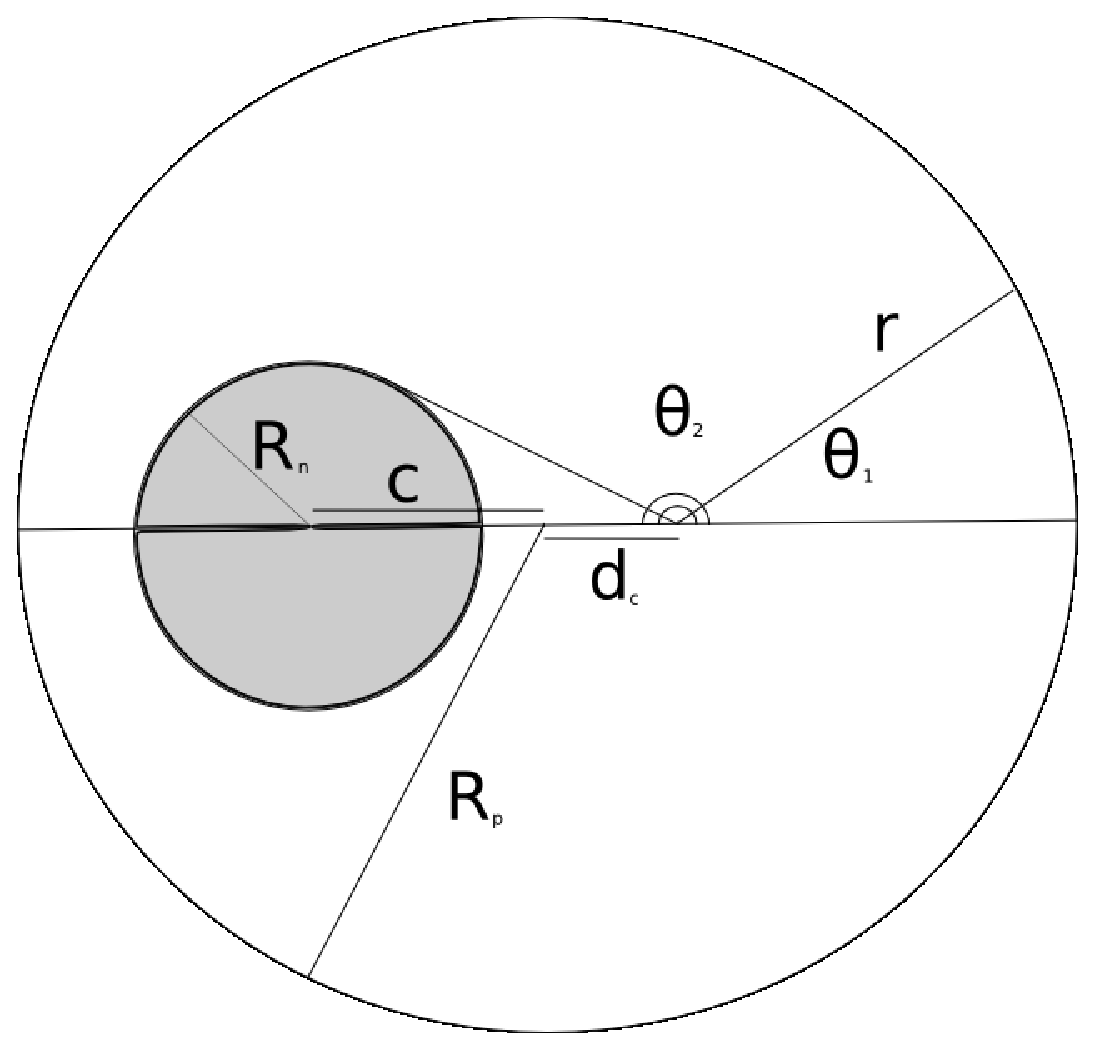
\includegraphics[width = .49\textwidth]{plots/figure_rhalf.eps}
\caption{\label{fig:geom_crescent} Geometry of crescent sources.}
\end{figure}





\section{Lightcurves of the extended sources during fold crossing}

Using equation \ref{eqn:ft} and the one-dimensional flux function presented in the previous section one can compute numerically the lightcurves of the three extented sources for the simplified 
infinite-wall-caustics model.

\subsection{Lightcurve of the gaussian source}

The amount of light received by an observer from a source with a gaussian distributed brightness with $\sigma$ and total flux $S_0^G$ in the absence of any gravitational lensing is:
\begin{equation}
 F^G(t) = \int_{-\infty}^\infty  \left( \mu_0 + \frac{C_0}{\sqrt{p}} \Theta \left( p \right) \right) \left( \frac{S_0^G}{\sqrt{2 \pi} \sigma} e^{-\frac{(p-p_s(t))^2}{2 \sigma^2}} \right) \mathrm{d}p.
\end{equation}

which can be simplified to:
\begin{equation}
 F^G(t) = \mu_0 S_0^G + \frac{C_0 S_0^G}{\sqrt{2\pi} \sigma} \int_{0}^\infty \frac{e^{-\frac{(p-p_s(t))^2}{2 \sigma^2}}}{\sqrt{p}} \mathrm{d}p.
\end{equation}



\begin{figure}
\centering
	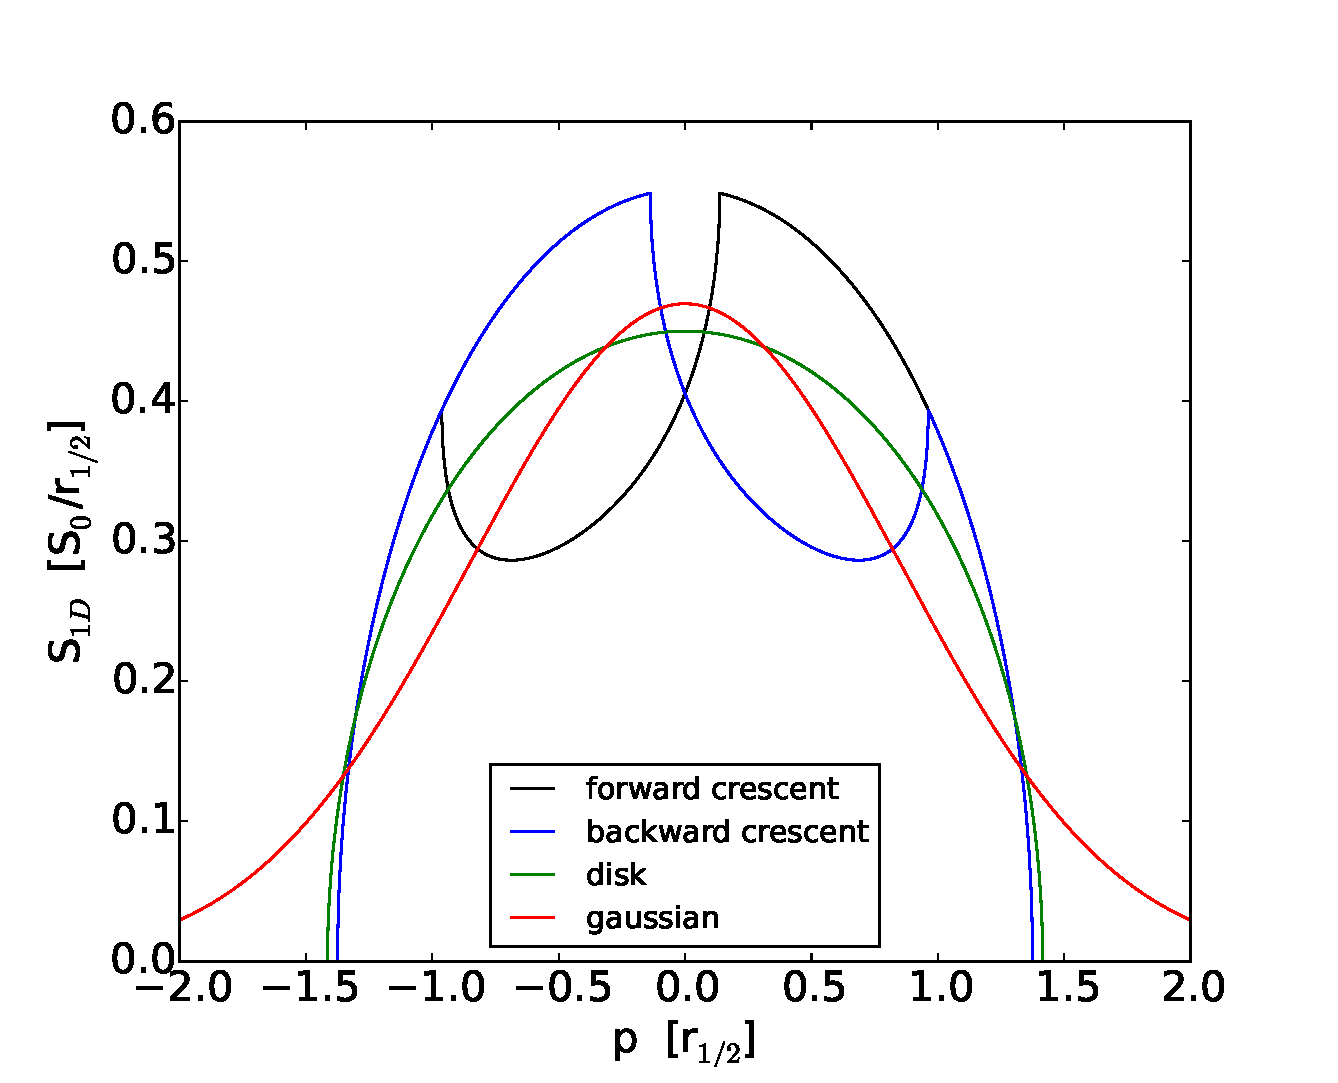
\includegraphics[width = 0.48\textwidth ,bb=0 0 576 520
	]{plots/S1D_all.eps}
	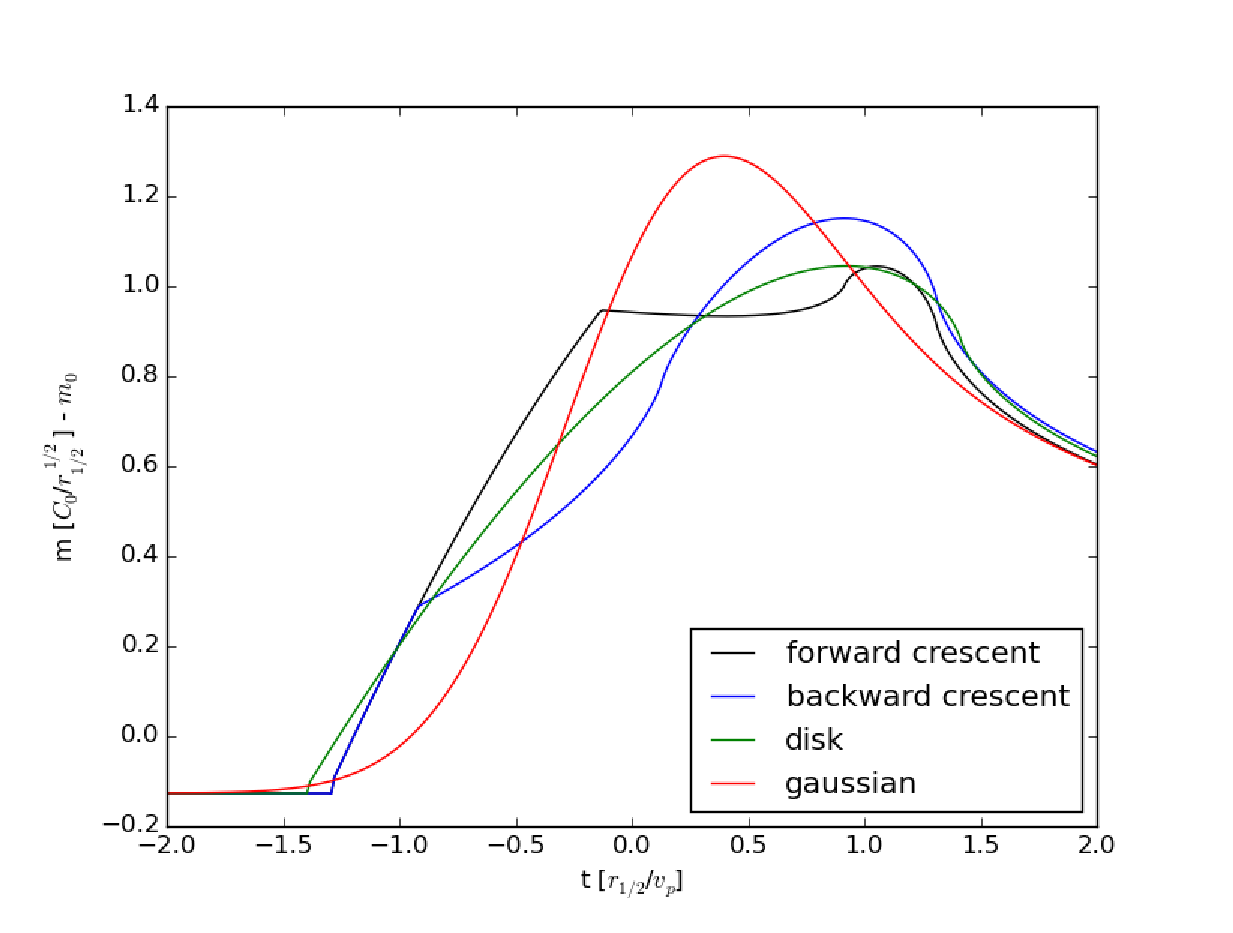
\includegraphics[width = 0.48\textwidth ,bb=0 0 576 520
	]{plots/4source_magnification.eps}
\caption{\label{fig:lightcurve_gauss} Lightcurves of crescents, Gaussian and disk for sources with identical $S_0$ and $r_{1/2}$. Crescent source has $r_{1/2}$ = 0.72754 $R_p$, $R_n$ = 0.4 $R_p$, a = 0.3/-0.3 $R_p$ }
\end{figure}


\subsection{Lightcurve of the disk shaped source}

Analogous to the gaussian shaped source, the disk source with uniform brightness, radius $R$ and unmagnified flux $S_0^D$ has a lightcurve described by the equation:

\begin{equation}
\begin{aligned}
 F^D(t) &= \int_{-\infty}^\infty  \left( \mu_0 + \frac{C_0}{\sqrt{p}} \Theta \left( p \right) \right) \\
	& \bigg[ \frac{2 S_0^D}{ \pi R} \sqrt{1 - \frac{\left( p-p_s(t) \right)^2}{R^2}}  \Theta \left(R^2 - \left(p-p_s(t) \right)^2 \right) \bigg] \mathrm{d}p.
\end{aligned}
\end{equation}

which is equivalent to:
\begin{equation}
 F^D(t) = \mu_0 S_0^D + \frac{2 C_0 S_0^D}{\pi R} \int_{max(0, p_s(t) - R)}^{max(0, p_s(t) + R)} \frac{1}{\sqrt{p}} \sqrt{1 - \frac{\left( p-p_s(t) \right)^2}{R^2}} \mathrm{d}p.
\end{equation}

\begin{figure}
\centering
	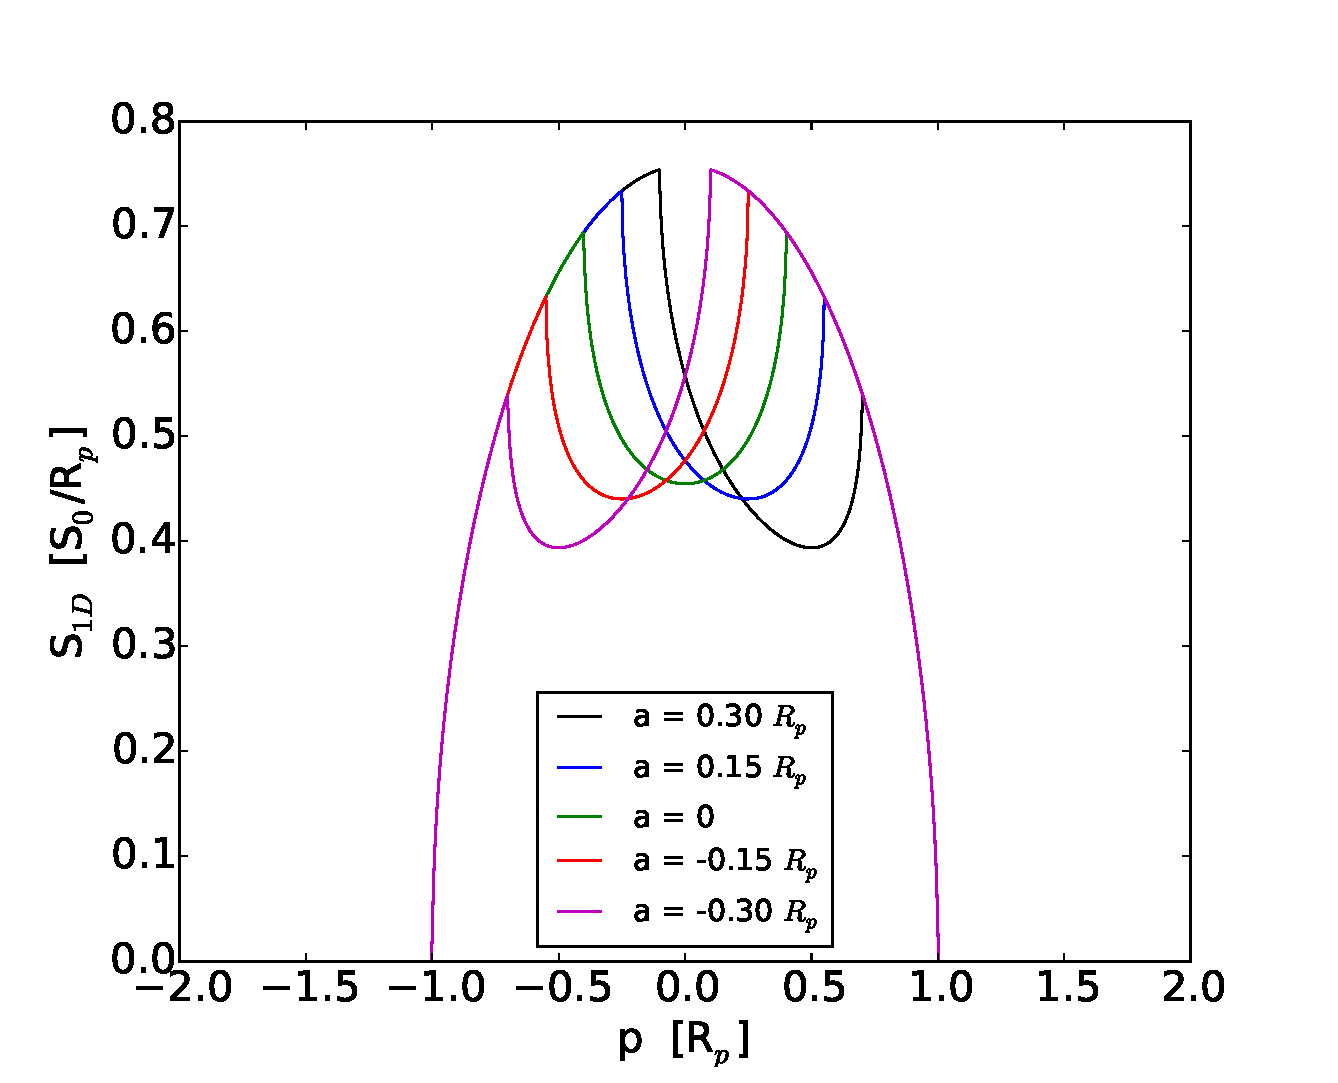
\includegraphics[width = 0.48\textwidth,bb=0 0 576 520
	]{plots/S1D_var_a.eps}
	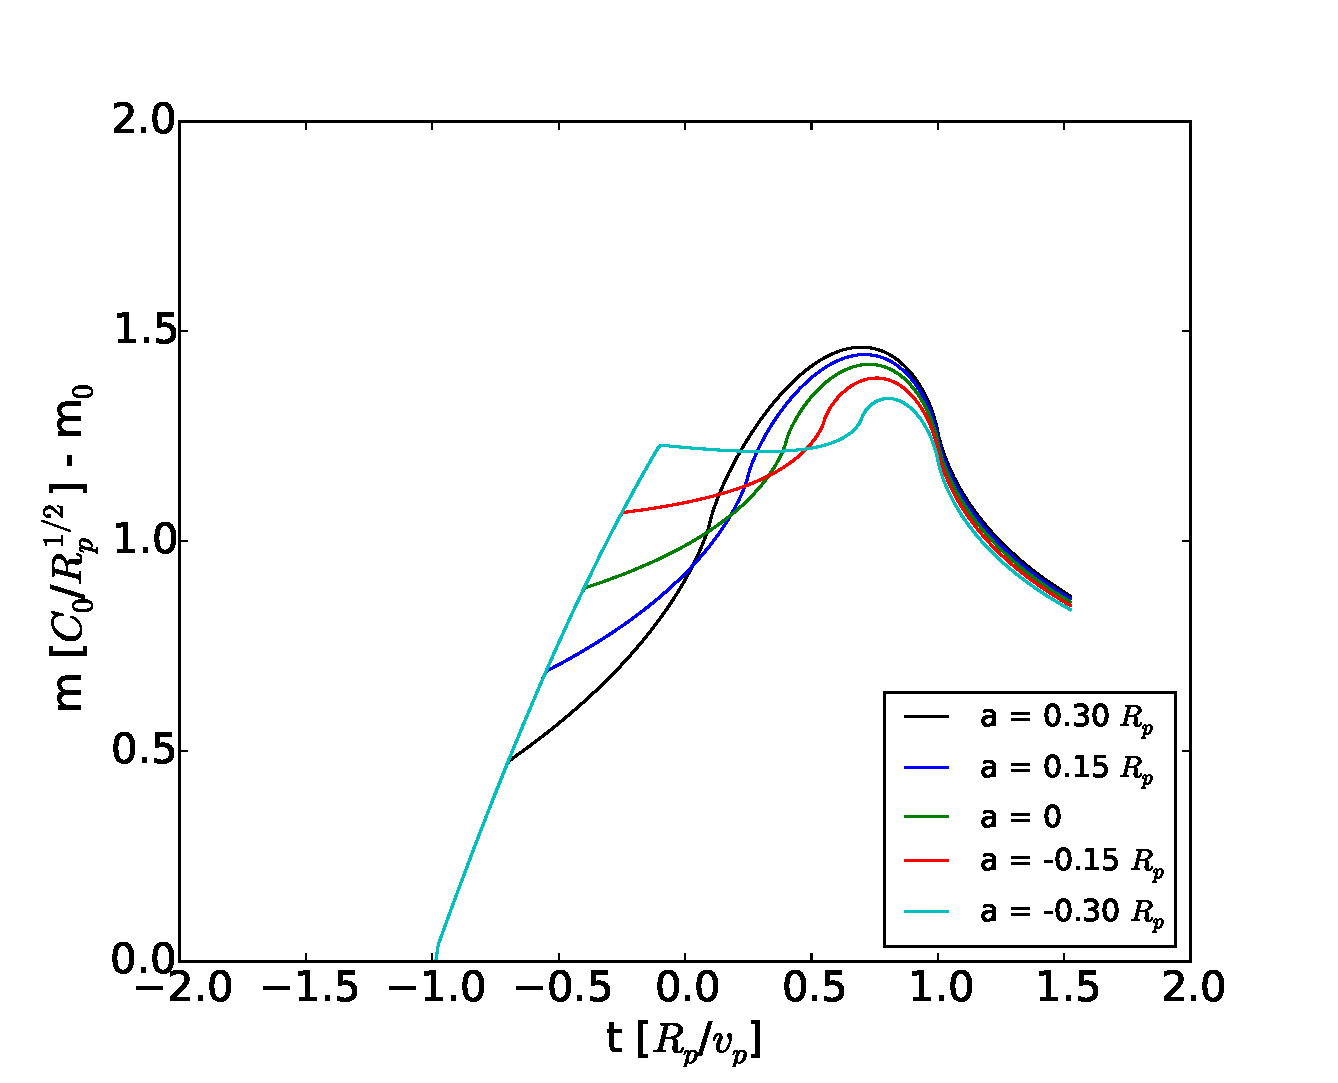
\includegraphics[width = 0.48\textwidth,bb=0 0 576 520
	]{plots/4avar_magnification.eps}
\caption{\label{fig:lightcurve_disk} Lightcurves of crescent sources with $R_n$ = 0.4 $R_p$.}
\end{figure}


\subsection{Lightcurve of the crescent shaped source}

The lightcurve of a crescent shaped source with unamplified flux $S_0^C$, radii $R_p$, $R_n$ and center displacement $a(t)$ is:


\begin{equation}
\begin{aligned}
 F^c(t) &= \mu_0 S_0^C + C_0 \frac{2 S_0^C}{\pi \left( R_p^2 -R_n^2 \right) } \\
	&\bigg[ \int_{max(0, p_s(t) - R)}^{max(0, p_s(t) + R)} \sqrt{\frac{R_p^2 - \left( p-p_s(t) \right)^2 }{p}} \mathrm{d}p \\
	&  -  \int_{max(0, p_s(t) - a(t) - R)}^{max(0, p_s(t) -a(t) + R)} \sqrt{\frac{R_p^2 - \left( p-p_s(t) +a(t) \right)^2 }{p}} \mathrm{d}p  \bigg] .
\end{aligned}
\end{equation}


\begin{figure}
\centering
	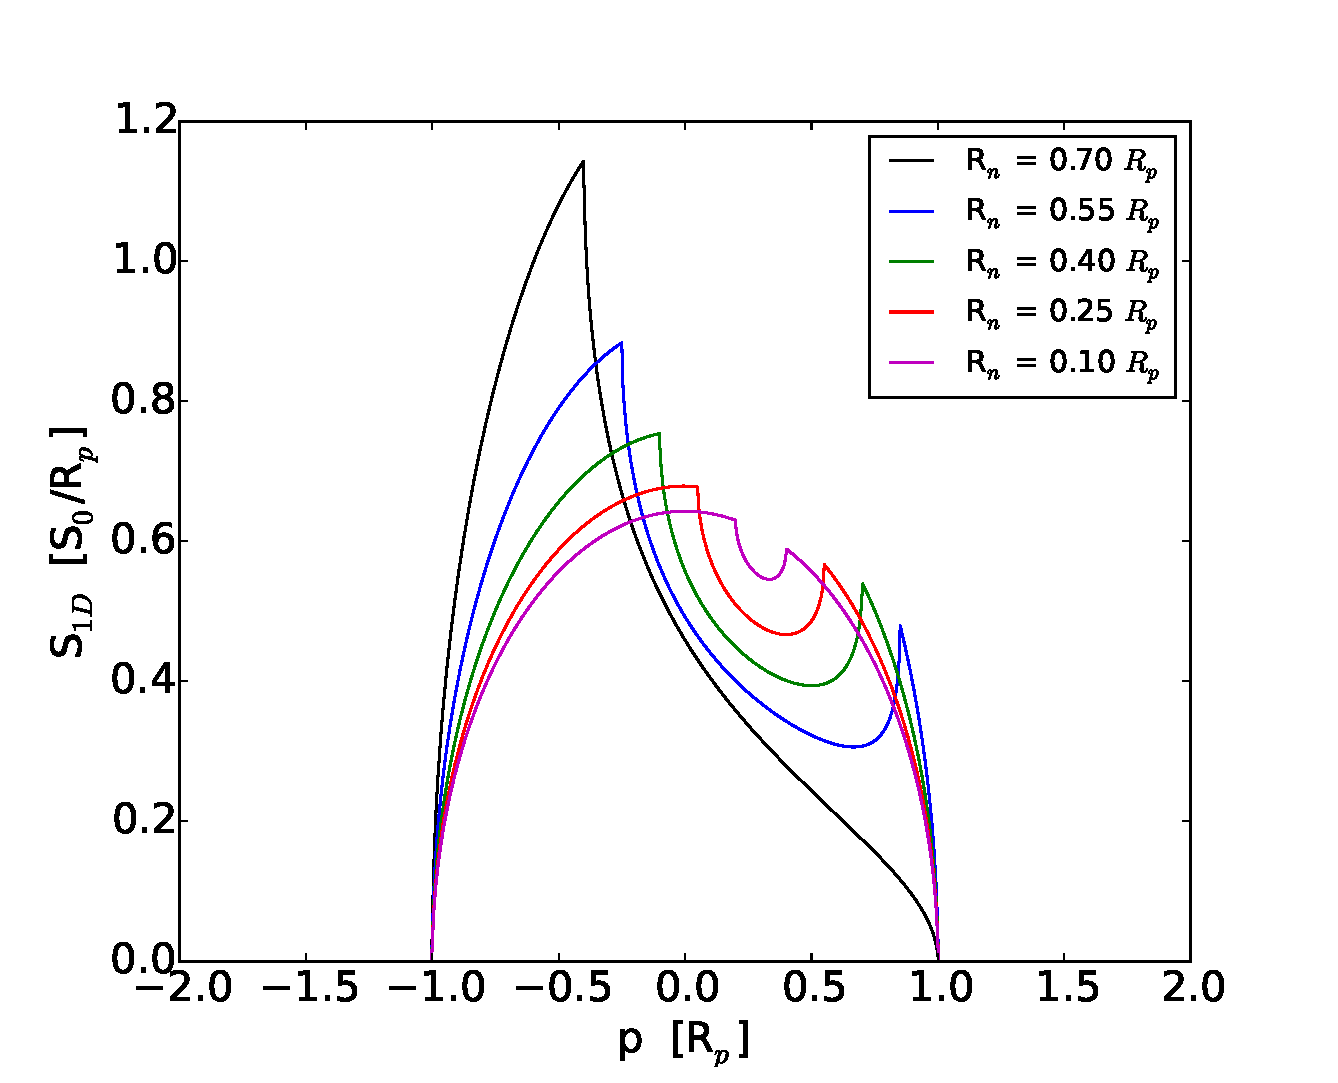
\includegraphics[width = 0.48\textwidth,bb=0 0 576 520
	]{plots/S1D_var_rn_a_poz.eps}
	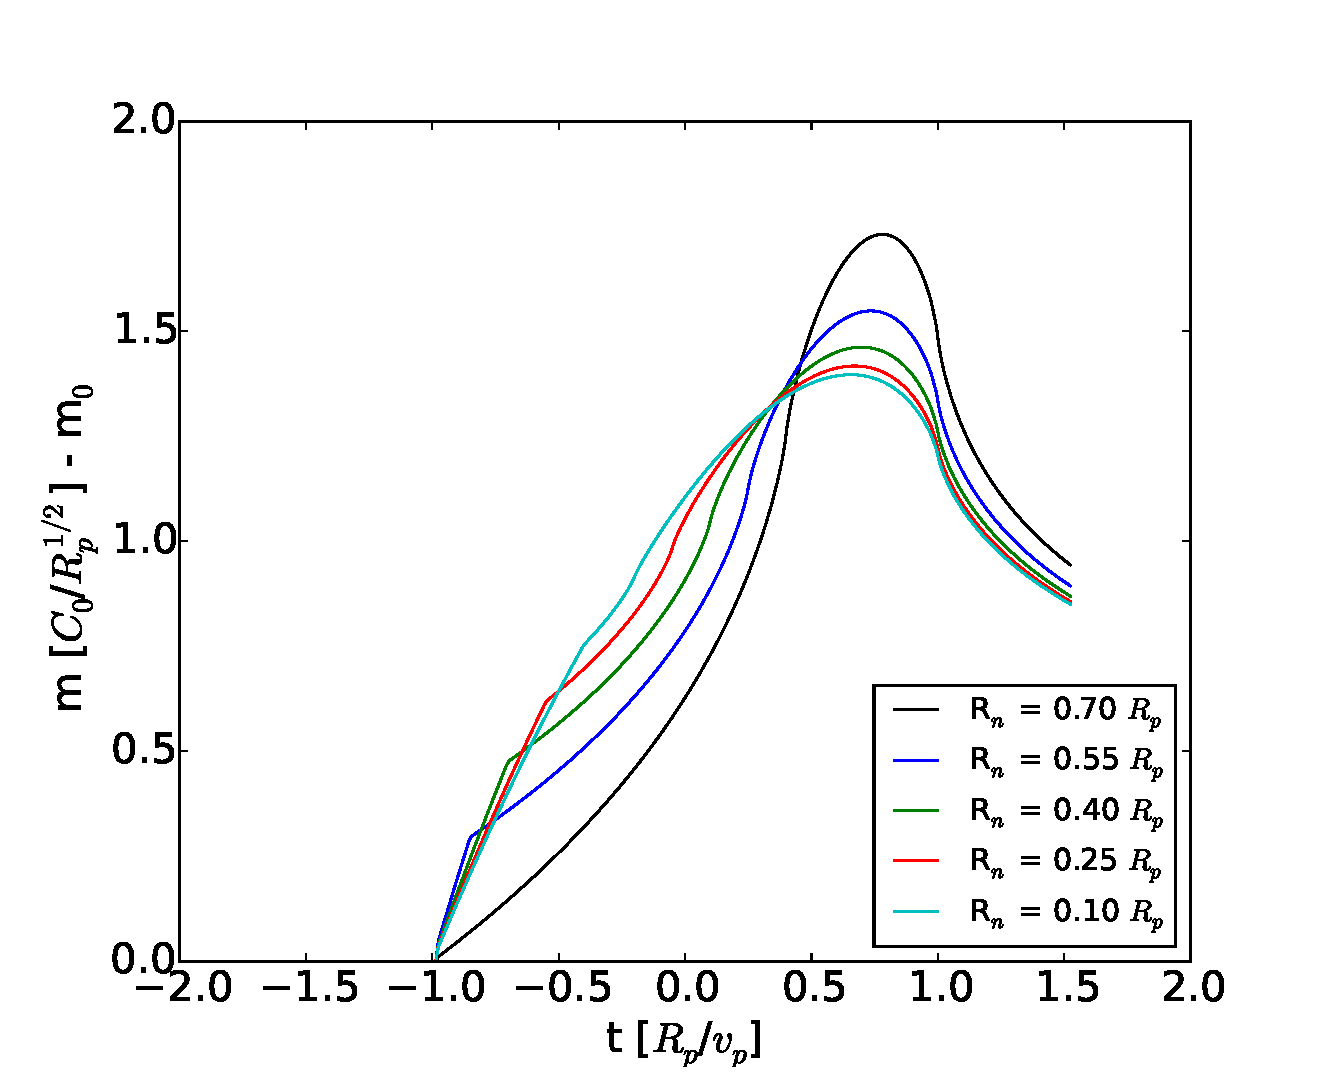
\includegraphics[width = 0.48\textwidth,bb=0 0 576 520
	]{plots/5Rn_back_var_magnification.eps}
\caption{\label{fig:lightcurve_crescent_back} Lightcurves of backwards crescents with  a = 0.3 $R_p$.}
\end{figure}

The function $p_s(t)$ can be chosen to be equal to $v_p(t-t_0) + p_{s0}$. Where $p_{s0}$ is the coordinate $p$ of the source at the initial time, and $v_p$ is the component of the velocity
along the $p$ axis. Such a modelling of the motion of the object in the source plane describes a linear motion with constant velocity. Furthermore, we reduce the complexity of the model by 
choosing the function $a(t)$ to be constant in time.  

\begin{figure}
\centering
	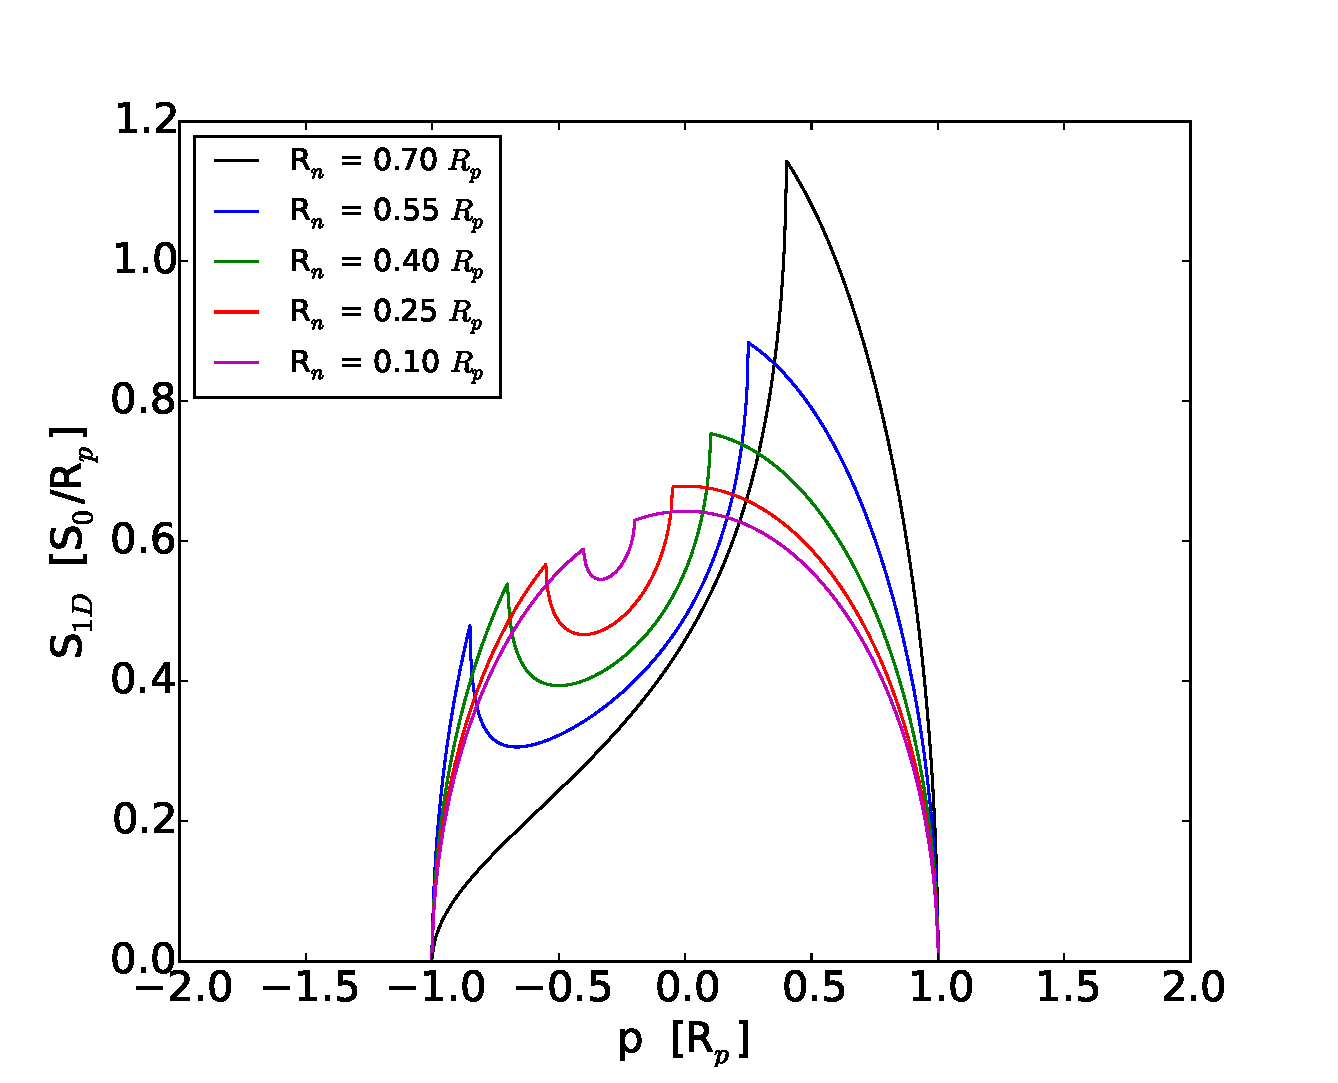
\includegraphics[width = 0.48\textwidth,bb=0 0 576 520
	]{plots/S1D_var_rn_a_neg.eps}
	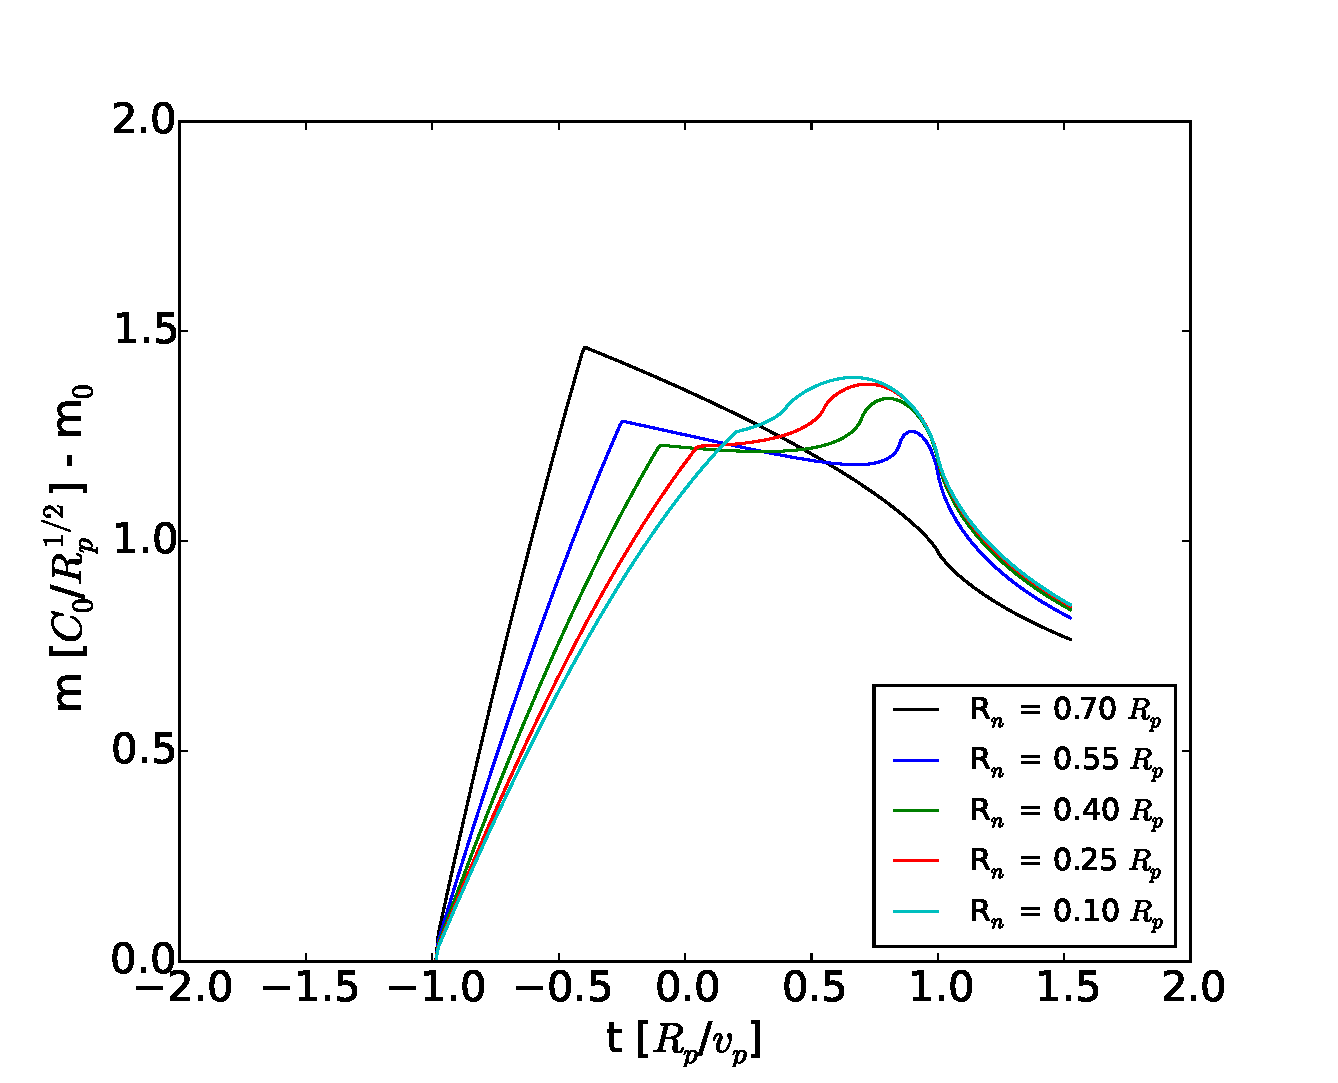
\includegraphics[width = 0.48\textwidth,bb=0 0 576 520
	]{plots/5Rn_forw_var_magnification.eps}
\caption{\label{fig:lightcurve_crescent} Lightcurve of forwards crescents with a = -0.3 $R_p$.}
\end{figure}

There are four characteristic points visible on the resulting one dimensional light profile of the crescent shaped source. Two of the points, p1 and p4, mark the outer boundaries of the luminous disc component. The other two, p2 and p3, mark the boundaries of the dark disc component. Since $S_1D$ is a projection of $S_2D$ on a line perpendicular to the caustic, the following relation holds:
\begin{equation}
	p_2-p_1 = R_p -R_n - a.
\end{equation}
In addition there are two other obvious relations the characteristic points which are independent of the projection:
\begin{equation}
	p_4 -p_1 = 2 R_p,
\end{equation}

\begin{equation}
        p_3 -p_2 = 2 R_n.
\end{equation}
All four points mark the positions where derivative $\frac{dS_{1D}}{dp}$ is discontinuous. The points can be used to define three regions: $p_1 - p_2$ where $S_1D$ is convex, $p_2 - p_3$ where $S_1D$ is concave, and $p_3 - p_4$ where $S_1D$ is convex again. \\

Due to the nature of the caustic and the monotonic behaviour of the magnification map on both sides of the caustic. The previously mentioned characteristic points are inherited by the microlensing lightcurve. The points on the temporal dimension $t_1, t_2, t_3$ and $t_4$ correspond to instances in time when the fold is aligned with $p_1, p_2, p_3$ and $p_4$, respectively. For a constant relative velocity $v_p$ between the source and the caustic there is a simple relation between the points $p_i$ and instances $t_i$:

\begin{equation}
	t_j - t_i = \frac{p_j - p_i}{v_p}.
\end{equation}

With the use of the previous four equations the following identities can be written:

\begin{equation}
	R_p = \frac{v_p \left( t_4 -t_1 \right)}{2}, 
\end{equation}

\begin{equation}
        R_n = \frac{v_p \left( t_3 -t_2 \right)}{2}, 
\end{equation}

\begin{equation}
        a = \frac{v_p \left( t_4 +t_1 - t_3 - t_2 \right)}{2}. 
\end{equation}



\begin{figure}
\centering
	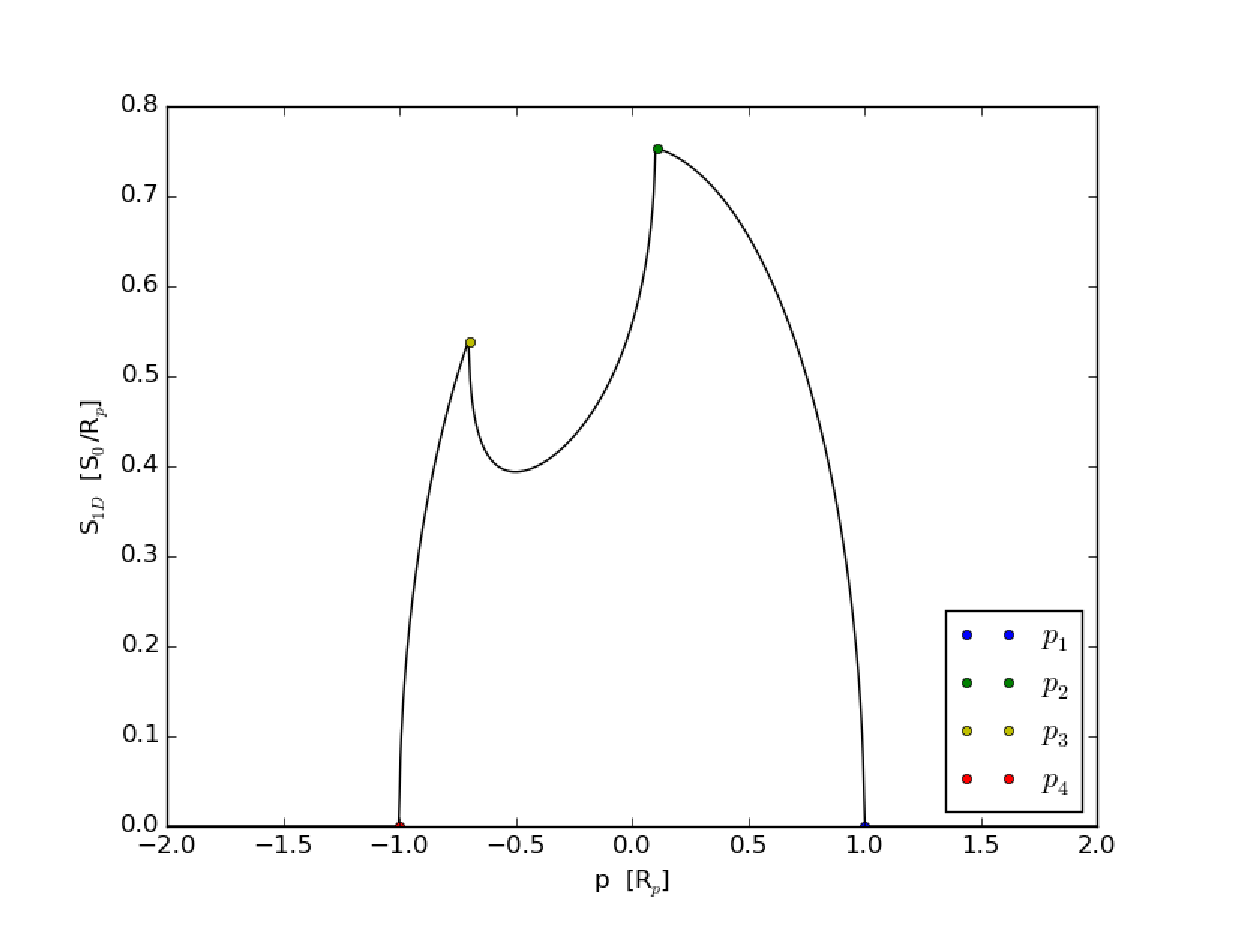
\includegraphics[width = 0.48\textwidth,bb=0 0 576 520
	]{plots/ch_points.eps}
        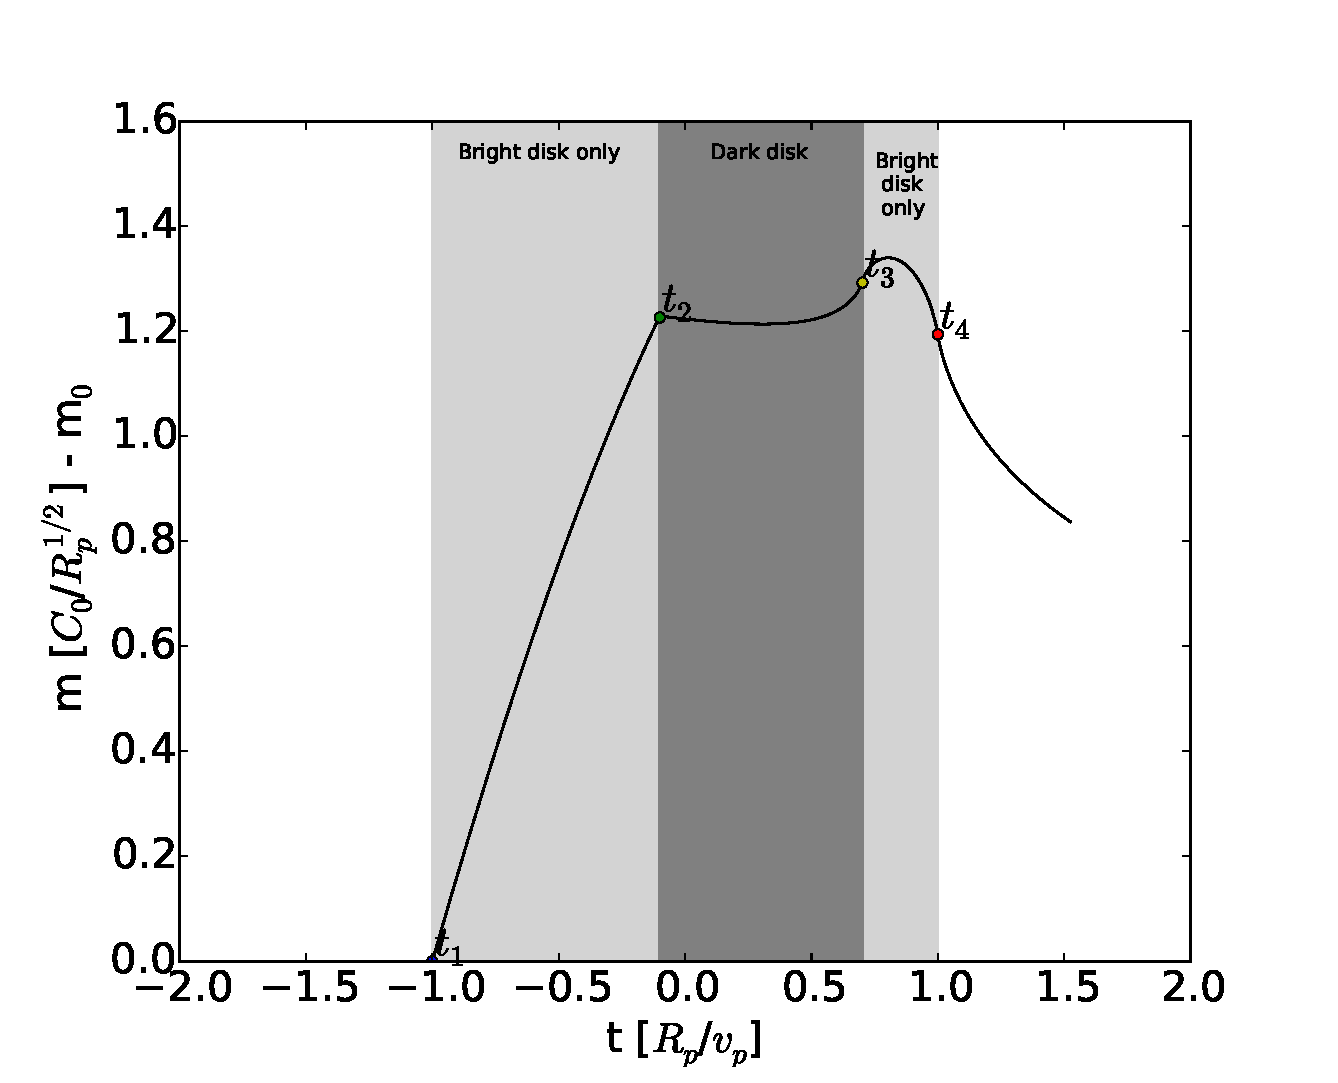
\includegraphics[width = 0.48\textwidth,bb=0 0 576 520
	]{plots/ch_instances.eps}
\caption{\label{fig:char_points} The characteristic points and instances of a crescent source's one dimensional profile and microlensing lightcurve. }
\end{figure}


Figure 4 reveals that the lighcurve of a crescent source has more visible features than the other two light-curves
corresponding to the disc and guasssian shape. There are three regions where $S_{1D}$ and by inheritance the lighcurve
 have distinguishable behaviour. The first region that would be recorded on a lightcurve plot represents the period
of time when the bright disk begins to be overlapped by the caustic and stops when just before the dark disk reaches
the caustic. During this period of time the flux of light from the source is increasingly magnified. The second
period starts and ends with the overlapping of the dark disc. As a boundary of the two regions there is a
distinguishable point where slope of the magnification is drastically changed. This apparent discontinuity in the
first derivative of the magnification function is caused by the caustic amplification of the sudden drop in the $S_{1d}$
function. During the respective period the magnification growth slows or even reverses during the first part of the
period and starts to grow faster again as the dark disk ends its overlap with the caustic. At the point where
the dark disc clears the caustic the growth of the magnification is infinite, which appears as a saddle point
on the lightcurve. Next, the final period correspond to the case when the dark disc has cleared the caustic
and the bright disc continues to overlap with the caustic. During this period the lighcurve reaches a peak
that for most of the parameter space is global and for the rest of the parameter space local.
At the end of the period the growth of the magnification is negative infinite. the respective point appears 
as a second saddle point on the lightcurve. Past this point the magnification of any finite source will 
decay in roughly the same manner. \\

The impact of parameter $a$ on the shape of the lightcurve can be observed in figure 5 (a-var). Sources where 
the center of the dark disc reaches the caustic before the center of the bright disc are characterized by a smoother
broad peak in contrast to the cases where the center of the dark disc reaches the caustic after the bright disk.
In the case of the latter the instance when the dark disc reaches the caustic corresponds to larger and
larger magnifications until it becomes a local and even global peak. The effect of the $R_n$  parameter on the
lighcurve is presented in figures 6 and 7. For the particular set of parameters where $R_p = R_n +a$ the third
period of time discussed previously does not exist. Particularizing further, if the value of the radius of the dark
disc is comparable to the value of the radius of the bright one then the position and shape of the maximum magnification
 are strikingly different. In case the crescent reaches the caustic with the bright region first, the peak magnification
 happens when the dark region reaches the caustic and it is characterized by a sharp variation in magnification growth,
In the opposite case the peak appears before the end of the bright disc reaches the caustic and shape is smoother. \\


\subsection{Microlensing a simulated image of M87}

\begin{figure}
\centering
        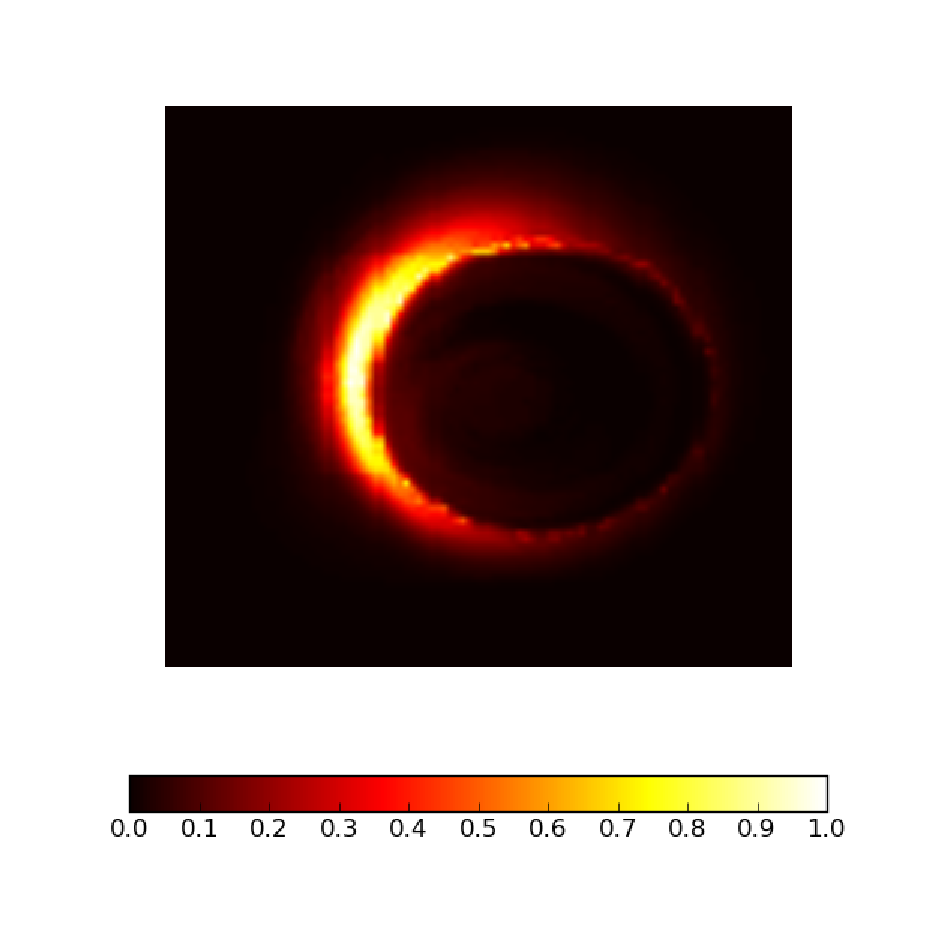
\includegraphics[width = 0.48\textwidth]{plots/M87_image.eps}
\caption{\label{fig:M87_image} The simulated image of M87's black hole sillouette obtained by \citep{2012MNRAS.421.1517D} from a GRMHD simulation presented in \citep{2009MNRAS.394L.126M}. The color bar is linear and scaled to reach value 1 for the maximum brightness. Points p2 and p3, mark the start and end of the equivalent dark disk and are associated to the moment of their overlap with the caustic t2 and t3.}
\end{figure}


\cite{2012MNRAS.421.1517D} have created a radiative image of M87 based on the GRMHD simulations presented in \citep{2009MNRAS.394L.126M}. The respective image, reproduced in figure \ref{fig:M87_image}, has been projected to a 1D profile associated to the perpendicular direction to a fold caustic approaching the image from the right. The projection is presented in the left panel of figure 10. The amplification values of the flux of light corresponding to a microlensing event are presented in the right panel of figure 10. In general the behaviour of the lightcurve is similar to the geometric crescent source with the caveat that the outer regions surrounding the luminous parts of the image have non-zero flux and thus are more extended than the simplified source model.

\begin{figure}
\centering
	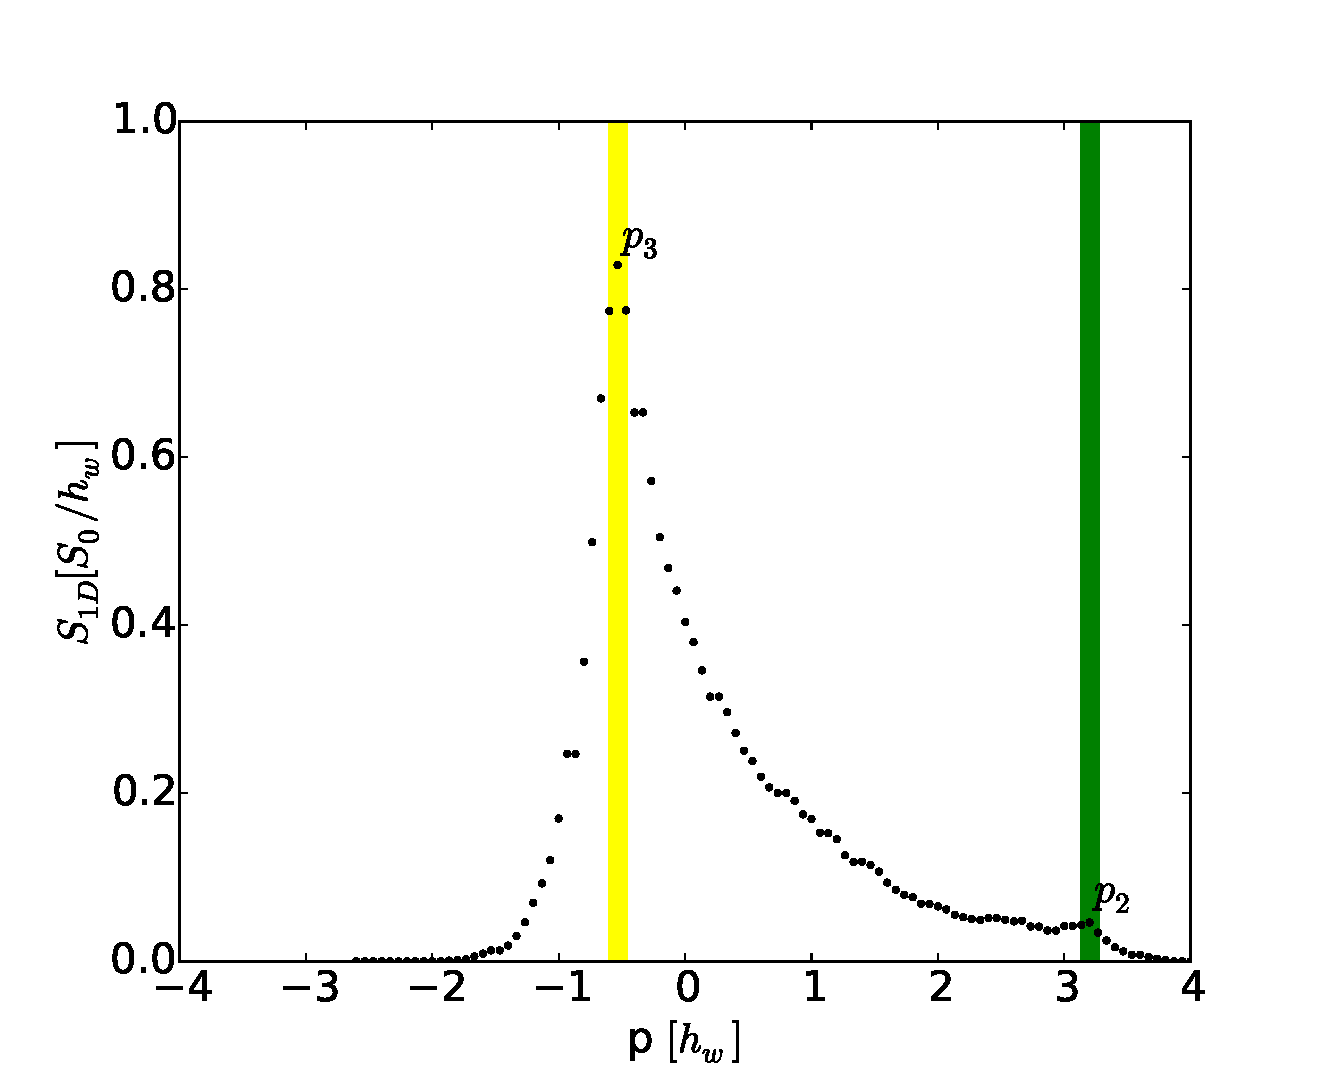
\includegraphics[width = 0.48\textwidth,bb=0 0 576 520
	]{plots/M87_shape.eps}
        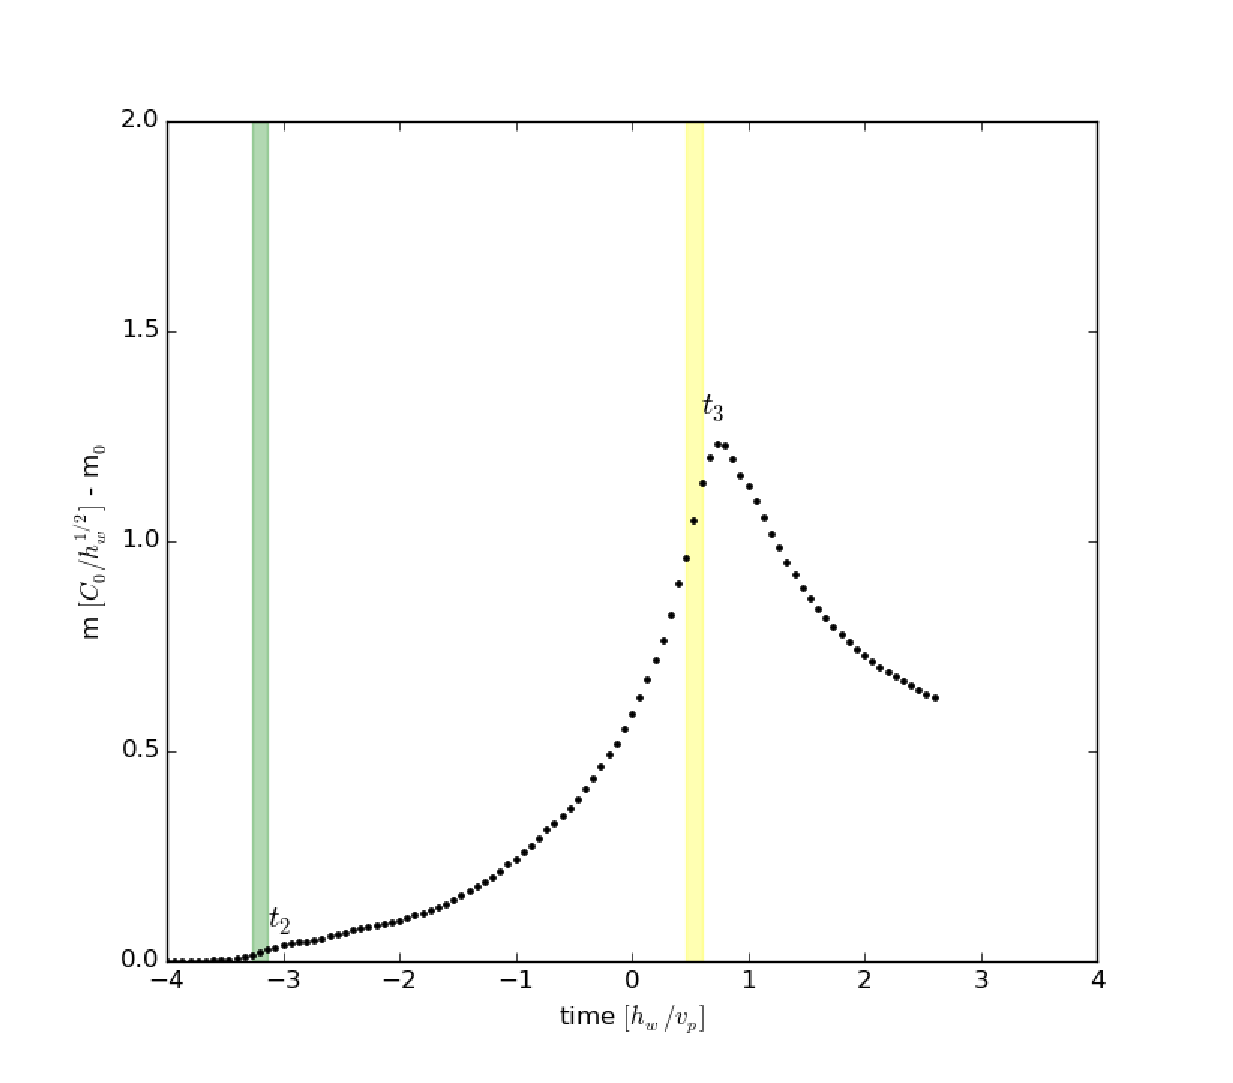
\includegraphics[width = 0.48\textwidth,bb=0 0 576 520
	]{plots/M87_lc.eps}
\caption{\label{fig:M87_plots} The one dimensional profile obtained from the numerical integration along the ordonata axis of the source image (figure 9) is presented in the left subplot. The corresponding lightcurve associated to the 1D profile is presented in the right subplot. The points p2 and p3 mark the start and end of the equivalent dark disk and are associated to the moments of their overlap with the caustic: t2 and t3.}
\end{figure}







\section{Microlensing code and magnification maps}
For the numerical computations of lightcurves for the models a and b, the microlensing code by Joachim Wambsgans was used, which is described in \cite{1999A&A...346L...5W}. This code is based on the hierachical tree technique to calculate the gravitational effect of the lensing masses. The underlying idea is that a microlensing situation can be separated into three planes, the observer, the lens plane and the source plane (assuming the thin lens approximation to be valid). The actual effect, namely the distortion of lightrays emitted from a distant source, on the way to the observer, is numerically computed by treating this situation from the opposite side: lightrays are shot backward from the observer to lens plane, where they become deflected according to the angle, which is given by the 2-dim. mass distribution in the lens plane.
\begin{equation}
\vec{\alpha}_{i}=\frac{4G}{c^{2}} \frac{D_{LS}}{D_{S}}\sum_{j=1}^{n}M_j \frac{\vec{r}_{ij}}{r^2_{ij}} 
\end{equation}  
For the computation of the individual deflection angles the tree idea is used. This means that the positions of all lensing masses are sorted into a 2-dimensional grid (in the lens plane). This grid is subdivided into 4 smaller squares until every cell contains only one mass. For the actual calculations of the deflection angle not every mass gravitational influence is treated equally. Instead it is made use of the fact that the influence of lenses on the considered lightray falls off with $r^{-1}$ from the point where the ray hits the lens plane. Hence masses situated at higher distances, can be grouped together in the calculation of their gravitational potential, by multipole moments. This way the amount of computation time is reduced. \\
When the deflection angles are determined, the deflected lightrays are traced to the source plane and a magnification map is created by counting the number of rays which hit each of its pixels. This is the inverse of what would happen in a real observation: here an observer on earth would detect light emitted by several sources with her/his telescope. Each of these sources emits lightrays which are subject to the deflection by the intervening gravitational potential of the lensing mass. However only a fraction of those will end in the observers telescope on earth. Interesting for the analysis are hence those lightrays which are originating by the source of interest and further the subset of these which actually converge at the location of the observer. So instead of calculating the trajectories of lightrays emitted by the source in all directions and then succeedingly pick out the ones which end in the telescope of the observer, the computational effort can be restricted to these lightrays of interest in the first place. This is done by treating the problem from the opposite direction, namely by using the observers location as starting point and then shooting the lightrays backwards till they hit the source plane. The result is a pixel map of the number of lightrays which arrive at the source plane. This intermediate result is denoted as the magnification map. It characterizes the information about the mass distribution in the lens plane and its effect on lightrays, and projects this information onto the source plane. \\\\
Once the map is created, the lightcurve can be obtained by specifying the transition path of the source within the map. The code thereby convolves the function describing the shape of the source with the magnification pattern of the map for each time step (see equation \ref{eqn:ft2d}). Note that in the most observational cases in microlensing, both lens and source are moving and further that the lens configuration, and with it the magnification pattern, is changing with time. While the first subtlety is taken care of by a coordinate transformation in this analysis, for the second one the lens configuration is assumed to be constant in time.  \\\\
For the model a it was desirable to work with a caustic geometry as simple as possible. Therefore only two equal point like masses were used as lenses, to produce the magnification map depicted in figure \ref{fig:magnification_map}. For a description of the parameter set which characterizes the map see (reference). The magnification maps calculated by the microlensing code are in units of Einstein radii, hence they are principally scale free. Physical scale is introduced to them by multiplying the pixels by the correct distance factor. The Einstein angle is given by   
\begin{equation}
\theta_{E}=\sqrt{\frac{4GM}{c^{2}} \frac{D_{LS}}{D_{S}D_{L}}} 
\end{equation}  
and therefore depends on the four parameters $M,D_{S},D_{L},D_{LS}$. For the cosmological application or quasar lensing $D_{L}$ is of order 100 Mps to Gpc and $D_{S}$ of order Gpc.\\   
The scale of the magnification map can be converted into a physical length by multiplying it by a factor of $ \sqrt{\frac{D_{LS}}{D_{S}D_{L}}}$.\\\\
For the next step, the computation of the actual lightcurve, the code was modified to also allow for crescent shaped images specified through the parameter set $R_p,R_n,a,b$. Here $R_p$ denotes the outer radius of the crescent and $R_n$ the inner one. The orientation of the source image with respect to the magnification map is specified by the parameters $a$ and $b$ as the shift of the center of the inner disk from the center of the outer disk in $x$- and $y$-direction respectively. In the original version of the code, gaussian and disk shaped images where already implemented. Those are completely characterized by the single parameter $R_p$. The values of the parameters are specified in pixel units corresponding to the magnification map. Further one needs to specify the start and end point coordinates of the path, which the center of the source image follows through the magnification map (see the depiction in figure \ref{fig:magnification_map}). Hence the points along this path are specified through the number of timesteps for which the computation of the brightness is to be carried out. Those points correspond to the actual measurement of the brightness of an object in the observational case. For each timestep the two-dimensional convolution of equation \ref{eqn:ft2d} is carried out numerically for the position of the source on the magnification map. \\
For the purpose of this analysis it was desirable to mimic the analytical behavior of a simple fold as much as possible, for comparing the numerical result with the analytical one, therefore the path of the source was chosen, so that it intersects the border of the caustic perpendicularly, and on a point where the border is almost straight.  


\section{Model fitting and likelihood analysis}

\begin{figure}
\centering
  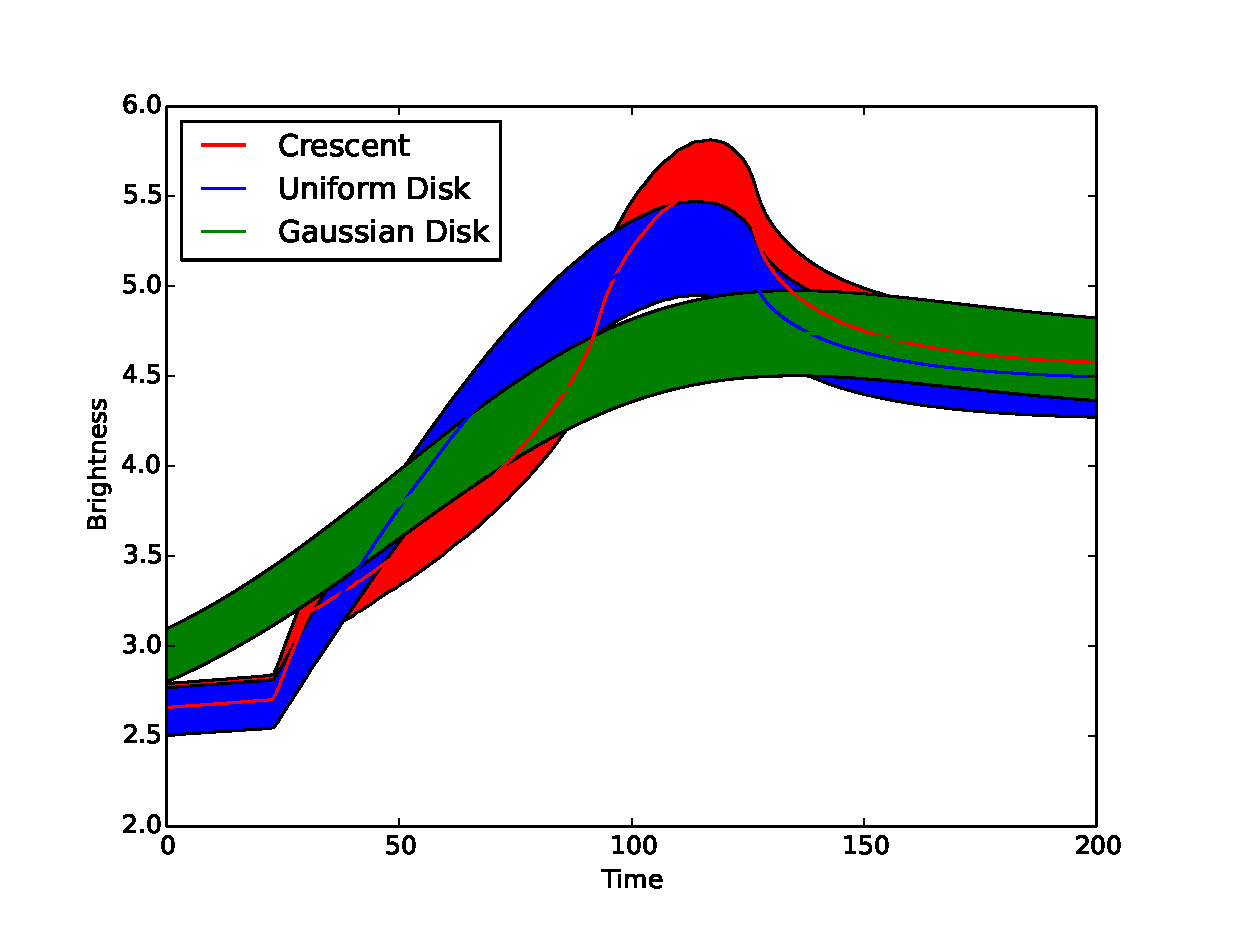
\includegraphics[width=0.95\hsize]{plots/data_with_error.eps}
\caption{\label{fig:datafitting} data}
\end{figure}


\begin{figure}
\centering
  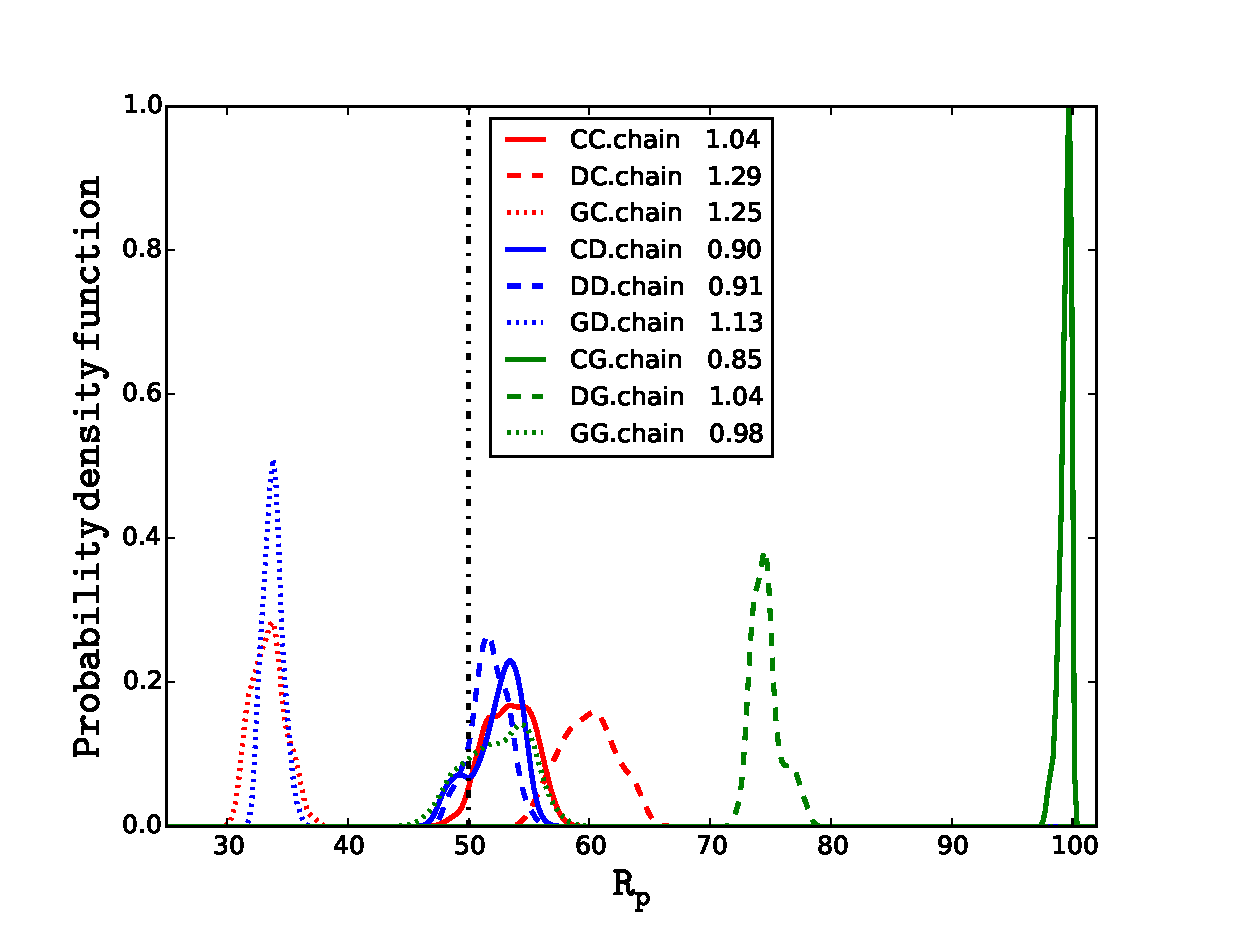
\includegraphics[width=0.45\hsize]{plots/Rp4all.eps}
  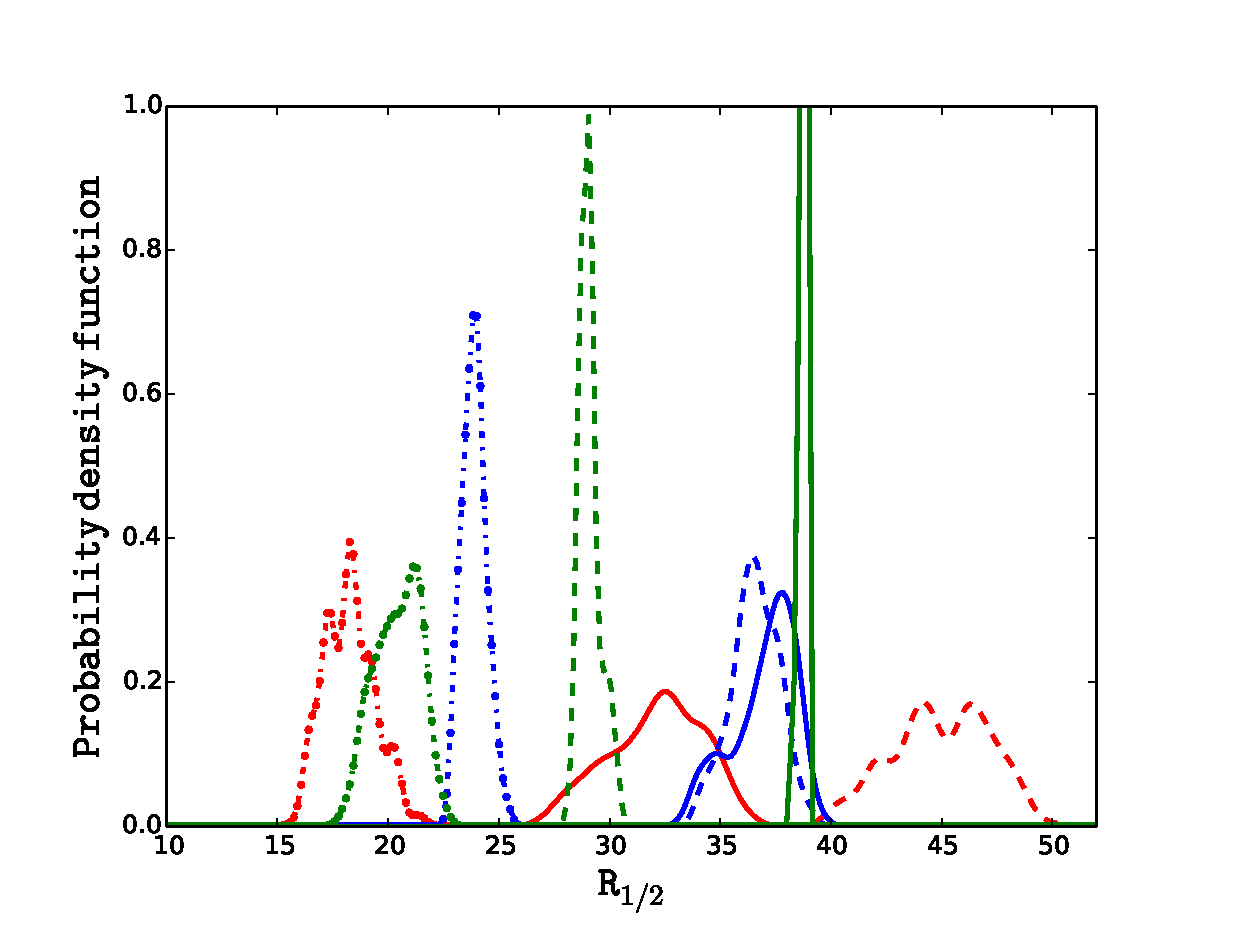
\includegraphics[width=0.45\hsize]{plots/Rhalf4all.eps}\\
  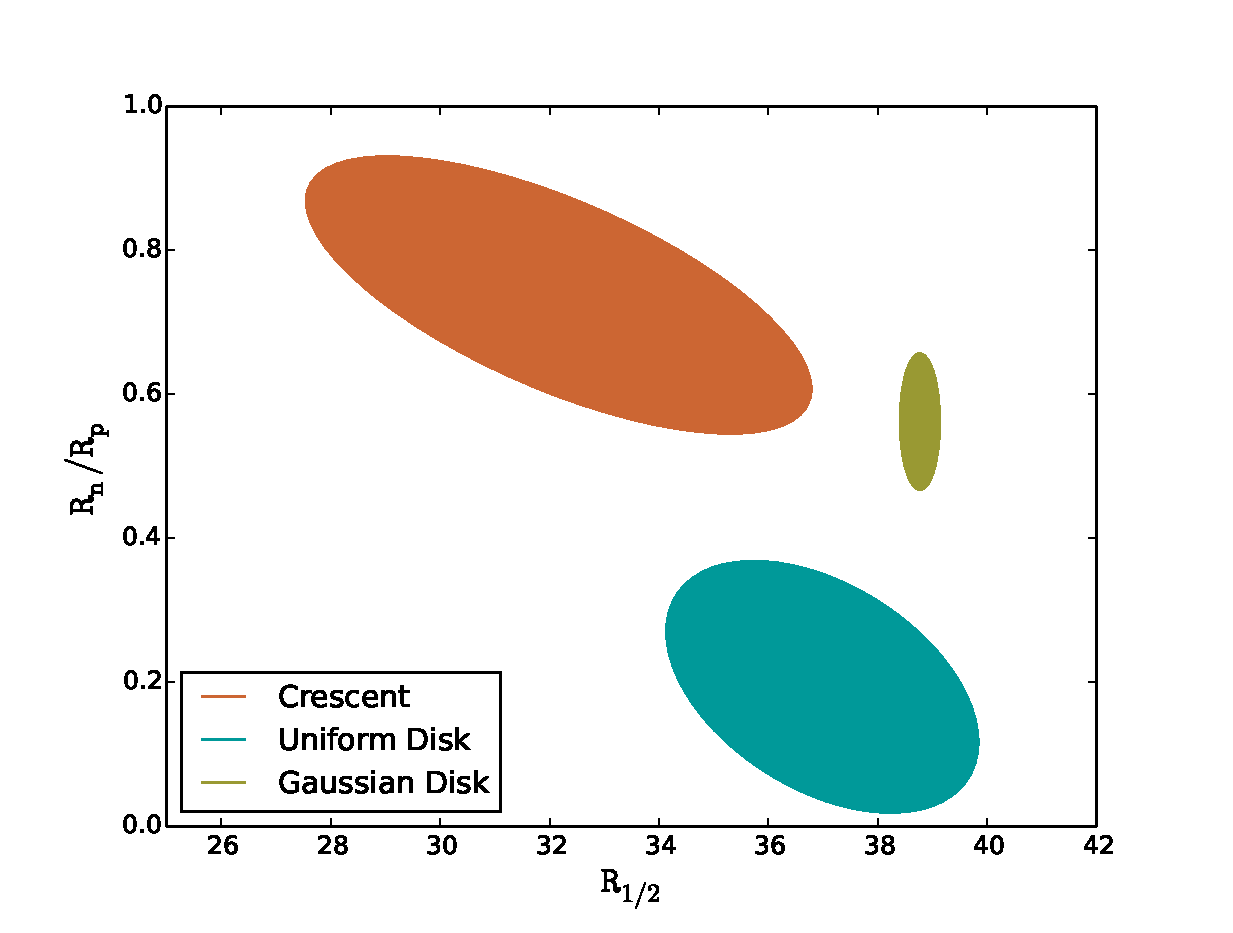
\includegraphics[width=0.45\hsize]{plots/Rhalf_RnRp.eps}
  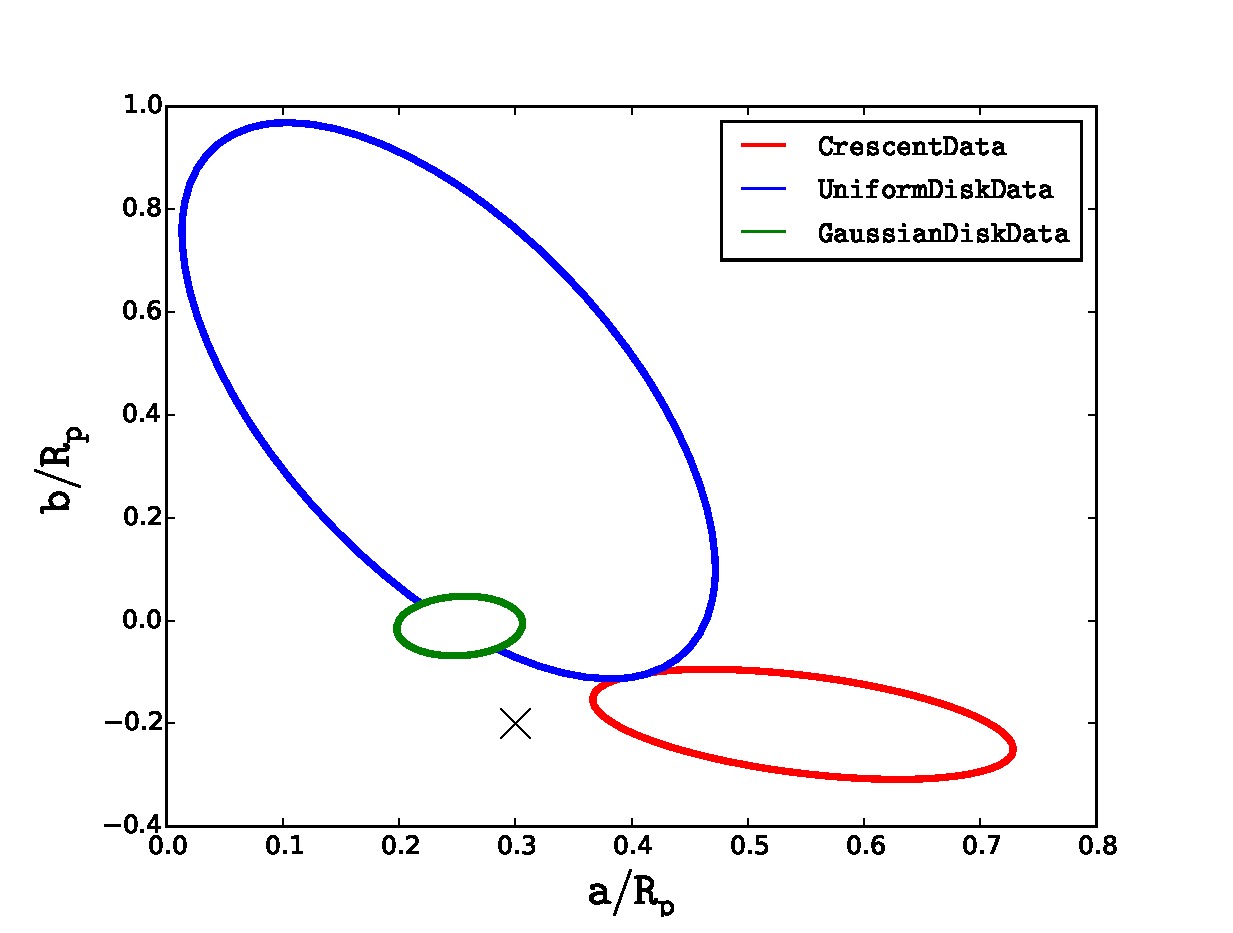
\includegraphics[width=0.45\hsize]{plots/aRp_bRp.eps}

\caption{\label{fig:mcmc} Model Fitting}
\end{figure}


In this section, we attempt to fit and recover the model parameters from the given dataset generated by different source models - crescent, uniform-disk and Gaussian-disk. So broadly we have 9 cases to discuss. We carried out a likelihood analysis on all three parameter set using Markov-chain Monte-Carlo (MCMC).

\subsection{Mock datasets}
The datasets for each source model is in the form of light curves, the brightness of the source observed at different time scale. Figure \ref{fig:datafitting} shows the three datasets. These datasets are generated using the magnification map shown in figure \ref{fig:magnification} between point B and C (direction from C to B). The data assumed was very  ideal, including 200 different data points at regular interval of time. It is worth noticing that the datasets generated using crescent model and uniform disc model resembles much more than the one generated by Gaussian disc model source. This is also very intuitive as uniform disc is a special case in crescent model where $R_n=0$, The fiducial model assumed to generate these mock datasets are:
\begin{equation}
	[R_p, R_n, a, b] = [50.0, 30.0, 15.0, 10.0]  \ \ \ \rm{for\ Crescent\ model},
	\label{eqn:cp}
\end{equation}
\begin{equation}
	R = 50.0 \ \ \ \rm{for\ Uniform\ disc\ model}
\end{equation}

\begin{equation}
	R = 50.0 \ \ \ \rm{for\ Gaussian\ disk\ model}
\end{equation}
\\
where, $R$ being the size of the uniform disc and Gaussian disc source model.

The aim of this exercise was to explore the degeneracies in  various model parameters and recover the correct fiducial model assumed. Also, it can be inferred if one can simply distinguish between circularly symmetric and asymmetric sources or uniform and Gaussian sources.
The errorbars on each data point, in all three datasets, is about 10 percent its value. Also, because we are fitting these datasets with different caustic crossing (point A to B in figure \ref{fig:magnification}), it adds a natural systematic errors on each data point. We also assume the errors are Gaussian distributed.


\subsection{Fitting with crescent model}
First we explored the parameter space for crescent source model and run its likelihood exploration for three different datasets. Here we have four parameters as given by equation \ref{eqn:cp}. Three red curves in top row of figure \ref{fig:mcmc} represents the resulting likelihood of $R_p$, the overall size of the crescent source for three different datasets. Solid red curve in top row and red contours in bottom row of figure \ref{fig:mcmc} represents the crescent fitting with crescent data (cc.chain in figure \ref{fig:mcmc}). All four parameters can be well recovered in this case and the overall likelihood coincides well with the fiducial values assumed and stated in equation \ref{eqn:cp}. It can also be well noticed that the half light radius is degenerate with $R_n/R_p$ or in other words, $R_p$ and $R_n$ are correlated.

In second case, we tried to fit crescent model to disk data (dc.chain in figure \ref{fig:mcmc}). The dashed red line in top row and blue contours in bottom row represents this case. Here one can recover the overall shape of the source, slightly lower than what is recovered in cc.chain case. Infact, the likelihood is higher than the previous case as the data is generated by one parameter only and fitting with four parameter that can also model the noise. Also, the maximum likelihood is achieved close to $R_n = 0$, as already mentioned, this is intuitive as well. The other paramters, $a$ and $b$ are quite arbitary. 

In the third case, Gaussian disc data is fit with crescent model (gc.chain). The dot-dashed red line in top row and green contours in bottom row represents this case. In this case, the extent of $R_p$ is broad and the likelihood is smaller than other cases.

Please notice that in top row of figure \ref{fig:mcmc}, the height of the peaks does not represents in likelihood, it is just ensuring that the area under the curve is unity. The likelihood can be estimated from the number in the legend which is the best $\chi^2$.

\subsection{Fitting with uniform disc model}
In this case, we have only one parameter to fit, the outer radius of the uniform disc with uniform intensity. When fitting with crescent data (solid blue line), the maximum likelihood shifts towards higher values of $R$ as compared to the fiducial value (which was 50). Also the maximum likelihood and is very low and the contraints are also very weak. However, when fitting with Gaussian disc (dot-dashed blue line), the likelihood is still very low, but the parameter is tightly constrained. The third case is ideal when fitting uniform disc data (blue dashed line), where the constraints are ideal and also co-incide well with the fiducial value assumed and also likelihood is comparatively better. 


\subsection{Fitting with Gaussian disc model}
In the last case, we fit Gaussian disc model to the three datasets (green curves in top row of figure \ref{fig:mcmc}). In this case, when fitted with Gaussian disc data, the likelihood coincide with the fiducial value assumed, in other cases the likelihood is away but weak and very well constrained. 


\section{Conclusion and interpretation}
The main results of this work is given in figure \ref{fig:mcmc} and described in the previous section. Here we try to interpret those results and conclude the take away message.

Lets assume that an ideal telescope observes a quasar for a long time and we get the lightcurve with good precision and one can clearly see the event of caustic crossing in the light curve. Now one wants extract the true shape of the source. To comment more specifically, lets assume three cases when the true shape of the source is: crescent, uniform disc and Gaussian disc:

\begin{enumerate}

\item Crescent shape source: if one tries to fit this curve with crescent model, the maximum likelihood will be good and one can recover the true parameters with good precision. In the other two cases, the maximum likelihood will be very bad. Hence this shape can be recovered very well by trusting the maximum likelihood analysis.
\item Uniform disc shape source: if one tries to fit this curve with Gaussian disk model, the likelihood will be very little to disprove it, however, the other two models are inditinguishable with nearly the same likelihood. At this point it does not matter as one can obtain the true result from both disk and crescent model.
\item Gaussian disc shape source: if one tries to fit this curve with uniform disk model, again likelihood will discard this choice. Again the maximum likelihood analysis will point towards the best fitted true model.

\end{enumerate}

At this point, we conclude that maximum likelihood analysis can be well trusted in order to recover true shape and recovering the corresponding parameters.

 


\section{Discussion}


\begin{itemize}
\item An interesting case for future study would be crescent model with Gaussian brightness profile.
\item More realistic errorbars and intervals of data points.
\item Experimenting with real data.
\item 

\end{itemize}





\bibliographystyle{mn2e}

\def\apj{ApJ}
\def\apjl{ApJL}
\def\aj{AJ}
\def\mnras{MNRAS}
\def\aap{A\&A}
\def\nat{nature}
\def\araa{ARAA}
\def\pasa{PASA}
\bibliography{heap}

\end{document}
